\chapter{Condensate Spectrum on the Freezeout Surface}

\section{Invariance of Fourier Transform w.r.t. Deformations of the Hypersurface}
\label{subsec:FourierDeformHypersurface}

Let $\phi_1,\phi_2$ be fields of equal mass evolving according to the KG equation. Then the current
\begin{equation}
    J_\mu[\phi_1,\phi_2]=-\imagu(\phi_1\partial_\mu\phi_2^*-(\partial_\mu\phi_1)\phi_2^*)\eqdef-\imagu\phi_1\overset{\leftrightarrow}{\partial_\mu}\phi_2^*
\end{equation}
with the antisymmetrized two-sided derivative $\overset{\leftrightarrow}{\partial_\mu}=\overset{\rightarrow}{\partial_\mu}-\overset{\leftarrow}{\partial_\mu}$ is conserved. Recall Gauß law on Cauchy hypersurfaces (up to a sign depending on the metric signature)
\begin{equation}
    \int_\Omega\dt \Omega\,\nabla^\mu J_\mu=\int_{\partial\Omega}\dt\sigma^\mu\,J_\mu
\end{equation}
with $\dt\sigma_\mu$ the outwards oriented surface normal of the spacetime volume $\Omega$. The bilinear form
\begin{equation}
    (\phi_1,\phi_2)_\Sigma=\int_\Sigma\dt\Sigma^\mu\,J_\mu[\phi_1,\phi_2]=-\imagu\int_\Sigma\dt\Sigma^\mu\,\phi_1\overset{\leftrightarrow}{\partial_\mu}\phi_2^*
\end{equation}
is therefore independent of the choice of (Cauchy) hypersurface $\Sigma$ (if $\partial\Sigma$ is changed, one must carefully check for further contributions in Gauß law).

Let 
\begin{equation}
    u_{\vec{p}}(t,\vec{x})=\exp(-\imagu(\omega_{\vec{p}}t-\vec{p}\vec{x}))\,,\qquad u_{\vec{p}}^*(t,\vec{x})=\exp(\imagu(\omega_{\vec{p}}t-\vec{p}\vec{x}))
\end{equation}
be the positive and negative frequency eigensolutions to the free Klein-Gordon equation. They form an orthogonal system with respect to the inner product defined above,
\begin{equation}
    (u_{\vec{p}},u_{\vec{q}})_{\Sigma_t}=(2\omega_{\vec{p}})(2\pi)^3\delta^{(3)}(\vec{p}-\vec{q})\,,\qquad (u_{\vec{p}}^*,u_{\vec{q}}^*)_{\Sigma_t}=-(2\omega_{\vec{p}})(2\pi)^3\delta^{(3)}(\vec{p}-\vec{q})\,,\qquad (u_{\vec{p}},u_{\vec{q}}^*)_{\Sigma_t}=0
\end{equation}
with the relations stated here on a a hypersurface $\Sigma_t$ where $t=\text{const.}$. This means that the Fourier coefficients, or equivalently annihilation and creation operators after quantization, for example in equation \eqref{eq:CanonicalQuant_RealScalar}, can be extraced via
\begin{equation}
    \sqrt{2\omega_{\vec{p}}}a_{\vec{p}}=(\phi,u_{\vec{p}})_{\Sigma_t}\,,\qquad \sqrt{2\omega_{\vec{p}}}a_{\vec{p}}^\dagger=-(\phi,u_{\vec{p}}^*)_{\Sigma_t}
\end{equation}
This leads of course to the same statement as in equations \eqref{eq:AnnCrePhiPi_Relation}.

Note how this has the form of the inner product defined in \ref{subsec:FourierDeformHypersurface}, to be precise
\begin{equation}
    a(\omega_{\vec{p}},\vec{p})=(\phi,e^{-\imagu(\omega_{\vec{p}}t-\vec{p}\vec{x})})_{\Sigma_t}\,,\qquad b(\omega_{\vec{p}},-\vec{p})=-(\phi,e^{\imagu(\omega_{\vec{p}}t-\vec{p}\vec{x})})_{\Sigma_t}
\end{equation}
and can therefore in principle be evaluated on any Cauchy surface.

In \cite{Amelino-CameliaEtAl_1997} it is argued that
\begin{subequations}
    \begin{align}
        \phi_{\text{out}}(t,\vec{p})&=\frac{1}{\omega_{\vec{p}}}\Big([\imagu \tilde{J}(\vec{p})]e^{-\imagu\omega_{\vec{p}}t}-[\imagu \tilde{J}(-\vec{p})]e^{\imagu\omega_{\vec{p}}t}\Big)\\
        \dot{\phi}_{\text{out}}(t,\vec{p})&=\Big(\tilde{J}(\vec{p})e^{-\imagu\omega_{\vec{p}}t}+\tilde{J}(-\vec{p})e^{\imagu\omega_{\vec{p}}t}\Big)
    \end{align}
\end{subequations}
    from which one derives \textbf{\textcolor{red}{prefactor of $2$?}}
\begin{subequations}
    \begin{align}
        \tilde{J}(\vec{p}) & =-\imagu e^{\imagu\omega_{\vec{p}}t}\big(\omega_{\vec{p}} \phi_{\text{out}}(t,\vec{p})+\imagu\dot{\phi}_{\text{out}}(t,\vec{p})\big)                                                                         \\
        \tilde{J}(-\vec{p})&=\imagu e^{-\imagu\omega_{\vec{p}}t}(\omega_{\vec{p}}\phi_{\text{out}}(t,\vec{p})-\imagu\dot{\phi}_{\text{out}}(t,\vec{p}))\\
        \intertext{By substition this gives}
        \tilde{J}(\vec{p}) & =-\imagu e^{\imagu\omega_{\vec{p}}t}\int\dt^3x\big(\omega_{\vec{p}}\phi(t,\vec{x})+\imagu\dot{\phi}(t,\vec{x})\big)e^{-\imagu\vec{p}\vec{x}}                                                                  \\
                           & =\int\dt^3x\big(\phi(t,\vec{x})\overset{\leftarrow}{\partial_t}e^{\imagu(\omega_{\vec{p}}t-\vec{p}\vec{x})}-\phi(t,\vec{x})\overset{\rightarrow}{\partial_t}e^{\imagu(\omega_{\vec{p}}t-\vec{p}\vec{x})}\big)\\
                           \intertext{and}
        \tilde{J}(-\vec{p})&=\imagu e^{-\imagu\omega_{\vec{p}}t}\int\dt^3x\big(\omega_{\vec{p}}\phi(t,\vec{x})-\imagu\dot{\phi}(t,\vec{x})\big)e^{-\imagu\vec{p}\vec{x}}\\
        &=\int\dt^3x\big(\phi(t,\vec{x})\overset{\leftarrow}{\partial_t}e^{-\imagu(\omega_{\vec{p}}t+\vec{p}\vec{x})}-\phi(t,\vec{x})\overset{\rightarrow}{\partial_t}e^{-\imagu(\omega_{\vec{p}}t+\vec{p}\vec{x})}\big)
    \end{align}
\end{subequations}
which, by the same argument as before, is independent of the choice of Cauchy surface.

The equations in \eqref{eq:SourceFieldRelation} are also precisely of this form, namely
\begin{subequations}
    \begin{align}
        J(p)&=-\int_{\Sigma_t}\dt\Sigma^\mu\,\phi_J\overset{\leftrightarrow}{\partial_\mu}u_{\vec{p}}^*=(\phi_J,u_{\vec{p}})_{\Sigma_t}\\
        J(-p)&=-\int_{\Sigma_t}\dt\Sigma^\mu\,\phi_J\overset{\leftrightarrow}{\partial_\mu}u_{\vec{p}}=(\phi_J,u_{\vec{p}}^*)_{\Sigma_t}
    \end{align}
\end{subequations}

We wish to evaluate this based on data given on the freezeout surface.\\
\debugbox{
    \begin{minipage}{\linewidth}
        \centering
        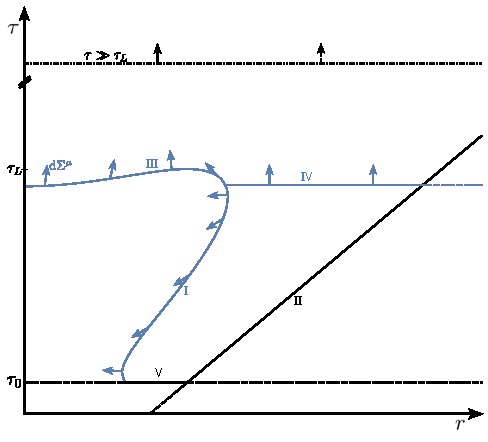
\includegraphics[width=0.4\linewidth]{images/FreezeOutSurface.pdf}
        \captionof{figure}{Freezeout surface in $\tau$-$r$-plane\cite{KirchnerEtAl_2023}.}
        \label{fig:FreezeOutSurface_rtau}
    \end{minipage}
}
Consider the freezeout on the hypersurface depicted in \ref{fig:FreezeOutSurface_rtau}. Assume that the condensate contribution as a function in phase space $f_{\text{cond}}(x^\mu,\vec{p})$ vanishes on $\Sigma_{\text{\rom{2}}}$ and $\Sigma_{\text{\rom{5}}}$, i.e. is contained within the union of all light cones starting on the freeze out surface $\Sigma_{FO}\equiv\Sigma_{\text{\rom{1}}}\cap\Sigma_\text{{\rom{3}}}$. \todo{By causality this seems reasonable, but from Fourier decomposition of a classical field this is not at all clear.} Following the reasoning from \cite{KirchnerEtAl_2023}, we wish to apply Gauß law, taking care of the different signature compared to the usual version of Gauß law in Euclidean space.

\begin{rmrk}[Gauß Law in Minkowski Space]{rmrk:GaußMinkowksi}
    From the Gauß law in Euclidean space
    \begin{equation}
        \int_\Omega\dt\Omega\,\vec{\partial}\cdot\vec{J}=\int_{\partial_\Omega}\dt\vec{\sigma}\cdot \vec{J}\,,
        \label{eq:GaußLawEuclidean}
    \end{equation}
    where ${\vec{\partial}\cdot\vec{J}\equiv\sum \partial_i J^i}$ is the divergence of $\vec{J}$, we wish to derive an analogous statement in Minkowski space, considering the differences in the metric signature. For simplicity, let the $\Omega$ be the region depicted in \ref{fig:GaußMinkowksi_Example} in a 1+1-dimensional spacetime with cartesian coordinates $(t,x)$. Assume the only relevant boundaries are parametrized by $x=x_\star=\const$ and $t=t_\star=\const$ and contributions at all other boundaries vanish.\\
\debugbox{
    \begin{minipage}{\linewidth}
        \centering
        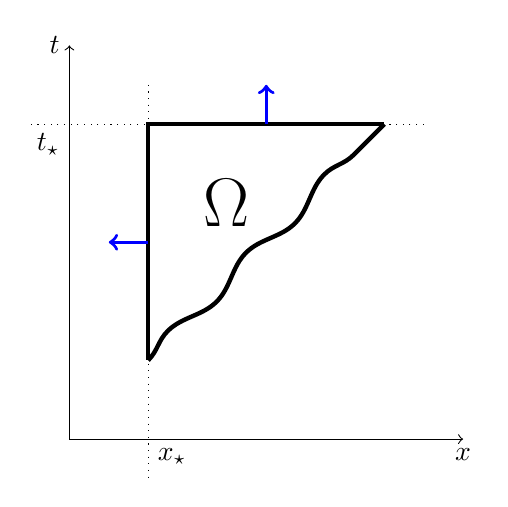
\begin{tikzpicture}
            \draw[->] (0,0) -- (5,0) node[below]{$x$};
            \draw[->] (0,0) -- (0,5) node[left]{$t$};
    
            \draw[ultra thick] (4,4) -- (1,4) -- (1,1);
            \draw[dotted] (4.5,4) -- (-0.5,4);
            \draw[dotted] (1,4.5) -- (1,-0.5);
            \draw[decorate,decoration={snake,segment length=40,post length=0},ultra thick] (1,1) -- (4,4);

            \draw[very thick, ->, blue] (1,2.5) -- (0.5,2.5);
            \draw[very thick, ->, blue] (2.5,4) -- (2.5,4.5);

            \node at (2,3) {\Huge$\Omega$};
            \node[anchor=north west] at (1,0) {$x_{\star}$};
            \node[anchor=north east] at (0,4) {$t_{\star}$};
        \end{tikzpicture}
        \captionof{figure}{Region of 1+1-dimensional spacetime with outwards oriented normal vectors (blue).}
        \label{fig:GaußMinkowksi_Example}
    \end{minipage}
}

    Denote $J^\mu\equiv\vec{J}\equiv(J^t,J^x)$ and calculate.
    \begin{subequations}
        \begin{align}
            \int_\Omega\dt\Omega\,\partial_\mu J^\mu&=\int_\Omega\dt\Omega(\partial_tJ^t+\partial_xJ^x)\\
            \intertext{\dots apply \ref{eq:GaußLawEuclidean}\dots}
            &=\int_{\partial\Omega}\dt\vec{\sigma}\cdot \vec{J}\\
            &=\int_{t=t_\star}\dt x\begin{pmatrix}
                1\\0
            \end{pmatrix}\cdot\begin{pmatrix}
                J^t\\J^x
            \end{pmatrix}
            +\int_{x=x^\star}\dt t\begin{pmatrix}
                0\\-1
            \end{pmatrix}\cdot\begin{pmatrix}
                J^t\\J^x
            \end{pmatrix}\\
            &=-\int_{t=t_\star}\dt x\begin{pmatrix}
                1\\0
            \end{pmatrix}\begin{pmatrix}
            -1&0\\0&1
            \end{pmatrix}\begin{pmatrix}
                J^t\\J^x
            \end{pmatrix}
            +\int_{x=x^\star}\dt t\begin{pmatrix}
                0\\-1
            \end{pmatrix}\begin{pmatrix}
                -1&0\\0&1
            \end{pmatrix}\begin{pmatrix}
                J^t\\J^x
            \end{pmatrix}
        \end{align}
    \end{subequations}
    which can be generalized to
    \begin{equation}
        \int_\Omega\dt\Omega\,\partial_\mu J^\mu=-\Big(\int_{\partial\Omega,\text{spacelike}}\dt\sigma^\mu\eta_{\mu\nu}J^\nu-\int_{\partial\Omega,\text{timelike}}\dt\sigma^\mu\eta_{\mu\nu}J^\nu\Big)
    \end{equation}
    Thus, unlike in the purely Euclidean case, there is a relative "-"-sign between contributions from spacelike and timelike boundaries in Minkowski space, as well as an overall "-"-sign due to the metric convention.
\end{rmrk}

Assuming that the condensate has no contributions at large rapidities $\eta\to\pm\infty$, one can deform the hypersurface $\Sigma_t$ at large lab time $t=\text{const.}$ into a hypersurface of large Bjorken time $\Sigma_{\tau\gg\tau_L}$ at a $\tau$ much larger then the lifetime $\tau_L$ of the fireball, using the Gauß law applied to the spacetime volume enclosed by these two Cauchy surfaces. The normal vectors have to be chosen with the same orientation.

Consider separately the contribution on the $\tau$-axis
\begin{equation*}
    \int_{\Sigma_{r=0}}\dt\Sigma^\mu\,J_\mu\qquad\text{or}\qquad\lim_{r\to 0}\int_{\Sigma_{r}}\dt\Sigma^\mu\,J_\mu
\end{equation*}
The surface vector on this hypersurface is $\dt\Sigma_\mu=r\tau\dt\tau\dt\eta\dt\varphi(0,1,0,0)$ and thus vanishes at $r=0$ (the hypersurface $\Sigma_{r=0}$ has zero $3$-volume). Since the derivative of a rotationally symmetric integrand introduces no divergencies, the contribution of $\Sigma_{r=0}$ to Gauß law is zero.

To conclude, the hypersurface on which the inner products are computed can be deformed according to
\begin{equation}
    (\phi_J,u_{\vec{p}}^{(*)})_{\Sigma_t}=(\phi,u_{\vec{p}}^{(*)})_{\Sigma_{\tau\gg\tau_L}}=(\phi,u_{\vec{p}}^{(*)})_{\Sigma_{\rom{3}}\cup\Sigma_{\rom{4}}}=(\phi,u_{\vec{p}}^{(*)})_{\Sigma_{\rom{3}}\cup\Sigma_{\rom{1}}}\equiv(\phi,u_{\vec{p}}^{(*)})_{\Sigma_{\text{fo}}}\,.
    \label{eq:InnerproductHypersurfaceDeformation}
\end{equation}
To verify the third equality in equation \ref{eq:InnerproductHypersurfaceDeformation}, one needs to recall the orientation of the normal vectors chosen in figure \ref{fig:FreezeOutSurface_rtau}, as well as an additional "-"-sign introduced by the timelike hypersurface $\Sigma_{\rom{1}}$.

\section{Coordinates on the Freezeout Surface}

The freezeout hypersurface is parametrized as $\Sigma_{\text{fo}}=\{x^\mu\in\mathbb{R}^{(1,3)}\vert (\tau,r)=(\tau(\alpha),r(\alpha))\}$ with $\tau,r$ defined by the coordinate transformation \eqref{eq:BjorkenCoords_PositionSpace}.

\begin{calc}[Metric on Hypersurface]{calc:HypersurfaceMetric}
    Recall the metric $g_{\mu\nu}=\text{diag}(-1,1,\tau^2,r^2)$ in coordinates $(\tau,r,\eta,\varphi)$. Orthonormal tangent vectors to the freeze out hypersurface are $(\hat\partial_\varphi)^\mu=(0,0,0,r^{-1})=r^{-1}(\partial_\varphi)^\mu$, $(\hat\partial_\eta)^\mu=(0,0,\tau^{-1},0)=\tau^{-1}(\partial_\eta)^\mu$ and $(\hat\partial_\alpha)^\mu=\sqrt{r^{\prime 2}(\alpha)-\tau^{\prime 2}(\alpha)}^{-1}(\tau^{\prime}(\alpha),r^{\prime}(\alpha),0,0)=D(\alpha)(\partial_\alpha)^\mu$ with $D(\alpha)=\sqrt{r^{\prime 2}(\alpha)-\tau^{\prime 2}(\alpha)}^{-1}$. The projector on the hypersurface is
    \begin{equation}
        \gamma_{\mu\nu}=(\hat\partial_\varphi)_\mu(\hat\partial_\varphi)_\nu+(\hat\partial_\eta)_\mu(\hat\partial_\eta)_\nu+(\hat\partial_\alpha)_\mu(\hat\partial_\alpha)_\nu=\begin{pmatrix}
            D^2(\alpha)\tau^{\prime2}(\alpha)               & -D^2(\alpha)\tau^\prime(\alpha)r^\prime(\alpha) & 0      & 0   \\
            -D^2(\alpha)\tau^\prime(\alpha)r^\prime(\alpha) & D^2(\alpha)r^{\prime2}(\alpha)                  & 0      & 0   \\
            0                                               & 0                                               & \tau^2 & 0   \\
            0                                               & 0                                               & 0      & r^2
        \end{pmatrix}
    \end{equation}
    The normal of the hypersurface is $n^\mu\equiv(\hat\partial_\alpha^\perp)^\mu=D(\alpha)(r^\prime(\alpha),\tau^\prime(\alpha),0,0)$ and is timelike where $D$ is real. Naturally $\gamma_{\mu\nu}n^\nu=0$. In the basis $(\partial_\alpha,\partial_\eta,\partial_\varphi,n)$ using (in short form)
    \begin{equation}
        (\partial_\alpha)^\nu\gamma_{\mu\nu}(\partial_\alpha)^\mu=\begin{pmatrix}
            \tau^\prime \\r^\prime
        \end{pmatrix}^T\begin{pmatrix}
            -\tau^\prime \\
            r^\prime
        \end{pmatrix}=D^{-2}
    \end{equation}
    the hypersurface metric in coordinates $x^i=(\alpha,\eta,\varphi)$ reads
    \begin{equation}
        \gamma_{ij}=\text{diag}(D^{-2}(\alpha),\tau^2(\alpha),r^2(\alpha))
    \end{equation}
    and the volume element is given by $\dt\Sigma=r(\alpha)\tau(\alpha) D^{-1}(\alpha)\dt\alpha\dt\eta\dt\varphi$. The oriented surface element is \begin{equation}
        \dt\Sigma^\mu=n^\mu\dt\Sigma=r(\alpha)\tau(\alpha)(r^\prime(\alpha),\tau^\prime(\alpha),0,0)\dt\alpha\dt\eta\dt\varphi
    \end{equation}
\end{calc}

It is also useful to evaluate $p_\mu x^\mu$ in the Bjorken coordinate system. Therefore introduce an analogous coordinate change in momentum space
\begin{equation}
    \left\{\begin{split}
        p^t&=m_T\cosh\eta_p\\
        p^z&=m_T\sinh\eta_p\\
        p^x&=p_T\cos\varphi_p\\
        p^y&=p_T\sin\varphi_p
    \end{split}\right.
\end{equation}
to rewrite the scalar product as
\begin{equation}
    p_\mu x^\mu\equiv-\tau(p^t\cosh\eta-p^z\sinh\eta)+r(p^x\cos\varphi+p^y\sin\varphi)=-\tau m_T\cosh(\eta-\eta_p)+r p_T\cos(\varphi-\varphi_p)
\end{equation}
We used the identities
\begin{equation}
    \cosh(a-b)=\cosh a\cosh b-\sinh a\sinh b\,,\qquad\cos(a-b)=\cos a\cos b+\sin a\sin b
\end{equation}
The integral measure changes according to $\dt^4p_{\text{cart}}=\dt m_T\dt p_T\dt\eta_p\dt\varphi_p\cdot m_T p_T$. The momentum shell condition $p^2+m^2=0$ is equivalently parametrized by $m_T^2=p_T^2+m^2\eqdef \omega_T^2$.

\section{Computing the Inner Product}

The projection of the derivative onto the surface normal of $\Sigma_{\text{FO}}$  is (omitting the $\alpha$-dependence) 
\begin{equation}
    \dt\Sigma^\mu\partial_\mu=(r^\prime\partial_\tau+\tau^\prime\partial_r)\cdot r\tau\,\dt\alpha\dt\eta\dt\varphi
\end{equation}
For the real scalar field $\pi^0$, following the ideas of section \ref{sec:FluidFromRealScalar}, one finds
\begin{equation}
    \dt\Sigma^\mu\partial_\mu=\chi(r^\prime \underbrace{u_\tau}_{\textcolor{red}{=-u^\tau}}+\tau^\prime u_r)\cdot r\tau\,\dt\alpha\dt\eta\dt\varphi
\end{equation}

It is useful to compute the following integrals related to Bessel functions: \url{https://dlmf.nist.gov/10.9}
\begin{subequations}
    \begin{align}
        \int_0^{2\pi}\dt\varphi e^{\pm\imagu a\cos\varphi}&=\int_0^{2\pi}\big(\cos(a\cos\varphi)\pm\imagu\sin(a\cos\varphi)\big)=2\int_0^\pi\cos(a\cos\varphi)\\
        &=2\pi J_0(a)\\
        \int_{-\infty}^\infty\dt\eta e^{\pm\imagu a\cosh\eta}&=2\int_0^\infty\dt\eta\big(\cos(a\cosh\eta)\pm\imagu\sin(a\cosh\eta)\big)\\
        &=\pi\big(-Y_0(a)\pm\imagu J_0(a)\big)\\
        &=\pm\pi\imagu(J_0(a)\pm\imagu Y_0(a))=\begin{cases}
            +\pi\imagu H^{(1)}_0(a)&\text{for "+"}\\
            -\pi\imagu H^{(2)}_0(a)&\text{for "-"}
        \end{cases}
    \end{align}
    Additionally to the integral representations, the following computation makes use of \url{https://dlmf.nist.gov/10.4}
    \begin{equation}
        J_{0}^\prime(x)=-J_1(x)\,,\qquad Y_0^\prime(x)=-Y_1(x)
    \end{equation}
\end{subequations}

\begin{subequations}
    \begin{align}
        J(\pm p) & =-\int_{-\infty}^\infty\dt\eta\int_0^{2\pi}\dt\varphi\int_0^\pi\dt\alpha\tau r\Bigg[\phi(\tau,r)\big(r^\prime\overset{\leftrightarrow}{\partial_\tau}+\tau^\prime\overset{\leftrightarrow}{\partial_r}\big)e^{\pm\imagu(\tau \omega_T\cosh(\eta-\eta_p)-r p_T\cos(\varphi-\varphi_p))}\Bigg] \\
                           & =-\int_{-\infty}^\infty\dt\eta\int_0^{2\pi}\dt\varphi\int_0^\pi\dt\alpha\tau r\Bigg[\phi(\tau,r)\big(r^\prime\overset{\leftrightarrow}{\partial_\tau}+\tau^\prime\overset{\leftrightarrow}{\partial_r}\big)e^{\pm\imagu(\tau \omega_T\cosh\eta-r p_T\cos\varphi)}\Bigg]                      \\
                           & =-2\pi^2\int_0^\pi\dt\alpha\tau r\Bigg[\phi(\tau,r)(r^\prime\overset{\leftrightarrow}{\partial_\tau}+\tau^\prime\overset{\leftrightarrow}{\partial_r})\Big[J_0(r p_T)\times\big(-Y_0(\tau\omega_T)\pm\imagu J_0(\tau\omega_T)\big)\Big]\Bigg]                                                 \\
                           & =2\pi^2\int_0^\pi\dt\alpha\tau r\Bigg[(r^\prime\partial_\tau+\tau^\prime\partial_r)\phi(\tau,r)\Big[J_0(r p_T)\times\big(-Y_0(\tau\omega_T)\pm\imagu J_0(\tau\omega_T)\big)\Big]+\nonumber                                                                                             \\
                           & \phantom{=}\qquad + \phi(\tau,r)\Big[\tau^\prime\times p_T J_1(r p_T)\times\big(-Y_0(\tau\omega_T)\pm\imagu J_0(\tau\omega_T)\big)+\nonumber                                                                                                                                       \\
                           & \phantom{=}\qquad\phantom{+\phi(\tau,r)\Big[}+r^\prime\times J_0(r p_T)\times\omega_T\big(-Y_1(\tau\omega_T)\pm\imagu J_1(\tau\omega_T)\big)\Big]\Bigg]
    \end{align}
\end{subequations}

\begin{subequations}
    \begin{align}
        J(\overset{(-)}{+}p) & =-\int_{-\infty}^\infty\dt\eta\int_0^{2\pi}\dt\varphi\int_0^\pi\dt\alpha\tau r\Bigg[\phi(\tau,r)\big(r^\prime\overset{\leftrightarrow}{\partial_\tau}+\tau^\prime\overset{\leftrightarrow}{\partial_r}\big)e^{\overset{(-)}{+}\imagu(\tau \omega_T\cosh(\eta-\eta_p)-r p_T\cos(\varphi-\varphi_p))}\Bigg] \\
                           & =-\int_{-\infty}^\infty\dt\eta\int_0^{2\pi}\dt\varphi\int_0^\pi\dt\alpha\tau r\Bigg[\phi(\tau,r)\big(r^\prime\overset{\leftrightarrow}{\partial_\tau}+\tau^\prime\overset{\leftrightarrow}{\partial_r}\big)e^{\overset{(-)}{+}\imagu(\tau \omega_T\cosh\eta-r p_T\cos\varphi)}\Bigg]                      \\
                           & =\overset{(+)}{-}2\pi^2\imagu\int_0^\pi\dt\alpha\tau r\Bigg[\phi(\tau,r)(r^\prime\overset{\leftrightarrow}{\partial_\tau}+\tau^\prime\overset{\leftrightarrow}{\partial_r})\Big[J_0(r p_T)\times H_0^{\overset{(2)}{(1)}}(\tau\omega_T)\Big]\Bigg]                                                 \\
                           & =\overset{(-)}{+}2\pi^2\imagu\int_0^\pi\dt\alpha\tau r\Bigg[(r^\prime\partial_\tau+\tau^\prime\partial_r)\phi(\tau,r)\Big[J_0(r p_T)\times H_0^{\overset{(2)}{(1)}}(\tau\omega_T)\Big]+\nonumber                                                                                             \\
                           & \phantom{=}\qquad + \phi(\tau,r)\Big[\tau^\prime\times p_T J_1(r p_T)\times H_0^{\overset{(2)}{(1)}}(\tau\omega_T)+r^\prime\times J_0(r p_T)\times\omega_T H_1^{\overset{(2)}{(1)}}(\tau\omega_T)\Big]\Bigg]
    \end{align}
\end{subequations}

\section{Models for Initial Data}

If $J^\mu_{V,A}$ are assumed to be parallel to $u^\mu$, the assumption that all fields change only in direction of $u^\mu$ is consistent.

We shall try to investigate certain classes of initial conditions:
\begin{impt}[Possibilies to Fix Initial Data]{impt:InitialData}
\begin{enumerate}
    \item prescribe fields and orhtogonal derivatives directly \dots
    \begin{itemize}
        \item \dots in the sense of an expansion (starting with constants, Gauß modes?, \dots)
        \item \dots as function of $(\tau,r)$
    \end{itemize}
    \item prescribe other physically accessible parameters like energy density $\epsilon$, pressure $p$, fluid velocity $u^\mu$\dots
\end{enumerate}
\end{impt}

\subsection{Real Fields}
\label{sec:FluidFromRealScalar}

Let $\phi$ be a real scalar field, e.g. $\phi\in\{\sigma,\pi^0\}$. The only availabe $4$-vector in the fluid theory is $u_\mu$. It is thus intuitive to try to identify the real-valued $4$vector $\partial_\mu\phi\sim u_\mu$. Taking the normalization $u_\mu u^\mu=-1$ into account, one finds
\begin{equation}
    u_\mu=\frac{\partial_\mu\phi}{\chi}\,,\qquad0<\chi^2\defeq-(\partial_\mu\phi)(\partial^\mu\phi)
\end{equation}
This does not restrict the initial data enough to uniquely specify the resulting spectrum. We are left to prescribe two functions on the freezeout surface, namely $\phi\vert_{\Sigma_{\text{fo}}}$ and $\chi\vert_{\Sigma_{\text{fo}}}$.

Regarding the second option in \ref{impt:InitialData}, from the fluid theory, we could try to match the energy density of the hypothetical superfluid
\begin{subequations}
    \begin{align}
        \epsilon_{s,\phi}=u_\mu u_\nu T^{\mu\nu}_{\phi}&=\frac{(\partial_\nu\phi)(\partial_\mu\phi)}{\chi^2}\Big((\partial^\mu\phi)(\partial^\nu\phi)+g^{\mu\nu}\big(-\frac{1}{2}(\partial_\alpha\phi)(\partial^\alpha\phi)-\frac{1}{2}m_\phi^2(\phi)^2\big)\Big)   \\
        &=\chi^2-\big(\frac{1}{2}\chi^2-\frac{1}{2}m_\phi^2\phi^2\big)  \\
        &=\frac{1}{2}\big(m_\phi^2\phi^2+\chi^2\big)
    \end{align}
\end{subequations}
which changes along the freezeout surface as
    \begin{equation}
        \dt\epsilon=m_\phi^2\phi\dt\phi+\chi\dt\chi=m_\phi^2\phi(\partial_i\phi)\dt^i s+\chi\dt\chi=m_\phi^2\phi(\chi u_i)\dt^i s+\chi\dt\chi
    \end{equation}
where the sum over $i\in\{\tau,r\}$ is to be taken w.r.t. to a Euclidean metric, i.e.
\begin{equation}
    \dt\phi=\dt\tau\partial_\tau\phi+\dt r\partial_r\phi=\dt\alpha(\tau^\prime \underbrace{u_\tau}_{\textcolor{red}{=-u^\tau}}+r^\prime u_r)\chi\equiv\chi u_i\dt^is
\end{equation}
with $\dt^i s=(\partial x^\mu)/(\partial\alpha)\dt\alpha\equiv(\tau^\prime,r^\prime)\dt\alpha$ the displacement vector on the freezeout surface. For this prescription, the solution $\phi$ on the freezout surface thus needs to fulfill the ODE
\begin{equation}
    \dt\phi=\chi u_i\dt^i s\,,\quad
    \dt\chi=\frac{1}{\chi}\dt\epsilon-m_\phi^2\phi u_i\dt^i s
\end{equation}
The solutions $(\phi,\chi)$ of this ODE have 1 degree of freedom, e.g. the ratio of kinetic energy $\epsilon_{\text{kin}}=(1/2)\chi^2$ and $\epsilon_{\text{pot}}=(1/2)m_\phi^2(\phi)^2$ at $\alpha=0$. To be precise, choose $r\in[0,1]$ and set $\epsilon_{\text{pot}}\big\vert_{\alpha=0}=r\epsilon$ and $\epsilon_{\text{kin}}\big\vert_{\alpha=0}=(1-r)\epsilon$.

\paragraph{The Sign of $u^\mu\partial_\mu\phi$}

The 4-vector $u^\mu$ is timelike, ${u_\mu u^\mu=-1}$ and future oriented, $u^\tau>0$. Long after the collision, when the fireball expands and density decreases, the amplitude of the condensate can be expected to decrease in direction of the fluid flow, ${\dt(\phi)^2\sim\phi\dt\phi<0}$ where
\begin{equation}
    \dt\phi=(u^\tau\partial_\tau\phi+u^r\partial_r\phi)\dt\tau_E=u^\mu\partial_\mu\phi\dt\tau_E
\end{equation}
with the eigen time interval $\dt\tau_E>0$. Inserting ${\partial_\mu\phi=\chi u_\mu}$ gives
\begin{equation}
    \dt\phi=\chi u_\mu u^\mu\dt\tau_E=-\chi\dt\tau_E\,.
\end{equation}
In this case, $\phi\chi>0$ is the appropiate choice for a decreasing density of the condensate in the frame of the expanding fireball.

\subsection{Complex Fields}

Let $\phi$ be a complex field, e.g. $\phi\in\{\pi^+,\pi^-\}$ with $U(1)$ symmetry. In the case of $\pi^\pm$, this $U(1)$ symmetry is the symmetry under chiral rotations of $\pi^1\leftrightarrow\pi^2$. Using $\pi^1=(1/\sqrt{2})(\pi^++\pi^-)$ and $\pi^2=(\imagu/\sqrt{2})(\pi^+-\pi^-)$, as well as $\pi^\pm=\sqrt{n}\exp(\pm\imagu\theta)$, the conserved current is
\begin{align}
    \epsilon^{a12}J_V^{a,\mu}&=(\partial^\mu\pi^1)\pi^2-(\partial^\mu\pi^2)\pi^1\\
    &=\frac{\imagu}{2}\Big((\partial^\mu\pi^++\partial^\mu\pi^-)(\pi^+-\pi^-)-(\partial^\mu\pi^+-\partial^\mu\pi^-)(\pi^++\pi^-)\Big)\\
    &=\imagu\Big(-(\partial^\mu\pi^+)\pi^-+(\partial^\mu\pi^-)\pi^+\Big)\\
    &=\imagu\sqrt{n}\Big(-\big((\partial^\mu\sqrt{n})+\imagu\sqrt{n}(\partial^\mu\theta)\big)+\big((\partial^\mu\sqrt{n})-\imagu\sqrt{n}(\partial^\mu\theta)\big)\Big)\\
    &=n(\partial^\mu\theta)
\end{align}

The ansatz $J_V^{\mu,a}\sim u^\mu$ now implies
\begin{equation}
    u^\mu=\frac{\partial^\mu\theta}{\chi_\theta}\,,\qquad 0<\chi_\theta^2\defeq-(\partial_\mu\theta)(\partial^\mu\theta)
\end{equation}
Further imposing $(\partial^\mu\pi^a)\sim u^\mu$ leads to 
\begin{equation}
    u_\mu=\frac{\partial_\mu\sqrt{n}}{\chi_n}\,,\qquad 0<\chi_n^2\defeq-(\partial_\mu\sqrt{n})(\partial^\mu\sqrt{n})
\end{equation}
and a resulting energy density of
\begin{subequations}
    \begin{align}
        \epsilon_{s,\phi}=u_\mu u_\nu T^{\mu\nu}_{\phi}&=\frac{(\partial_\mu\theta)(\partial_\nu\theta)}{\chi_\theta^2}\Big(2(\partial^\mu\phi)(\partial^\nu\phi^*)+g^{\mu\nu}\big(-(\partial_\alpha\phi)(\partial^\alpha\phi^*)-m_\phi^2\phi\phi^*\big)\Big)\\
        &=n\chi_\theta^2+\chi^2_n+m_\phi^2n
    \end{align}
\end{subequations}
where the intermediate calculation
\begin{subequations}
    \begin{align}
        (\partial^\mu\phi)(\partial^\nu\phi^*)&=\big((\partial^\mu\sqrt{n})+\imagu\sqrt{n}(\partial^\mu\theta)\big)\big((\partial^\nu\sqrt{n})-\imagu\sqrt{n}(\partial^\nu\theta)\big)\\
        &=(\partial^\mu\sqrt{n})(\partial^\nu\sqrt{n})+n(\partial^\mu\theta)(\partial^\nu\theta)+\imagu\big(\sqrt{n}(\partial^\mu\theta)(\partial^\nu\sqrt{n})-\sqrt{n}(\partial^\nu\theta)(\partial^\mu\sqrt{n})\big)\\
        (\partial_\mu\phi)(\partial^\mu\phi^*)&=-\chi_n^2-n\chi_\theta^2
    \end{align}
\end{subequations}
is useful. Note how the imaginary part of this tensor is antisymmetric and thus does not contribute upon contraction with a symmetric tensor.

Considering the fact that we have already proposed ways to initialize the real valued fields $\pi^1$, $\pi^2$, we could also just simply construct $\pi^\pm=(1/\sqrt{2})(\pi^1\mp\imagu\pi^2)$ from these fields. Given $\partial^\mu\pi^{1,2}$, the density of the charged pion fields changes as
\begin{equation}
    \partial^\mu n=\partial^\mu(\pi^+\pi^-)=\frac{1}{2}\partial^\mu\big((\pi^1)^2+(\pi^2)^2\big)=(\partial^\mu\pi^1)\pi^1+(\partial^\mu\pi^2)\pi^2
\end{equation}

\section{Examplary Spectra}

This section is aimed toward finding some intuition for the relation between particle mass, initial conditions and resulting spectra.

First, investigate the spectrum of a real scalar field for constant values of the field an normal derivative.\\
\debugbox{
    \begin{minipage}{\linewidth}
        \centering
        \debugbox{
            \begin{minipage}{0.45\linewidth}
                \centering
                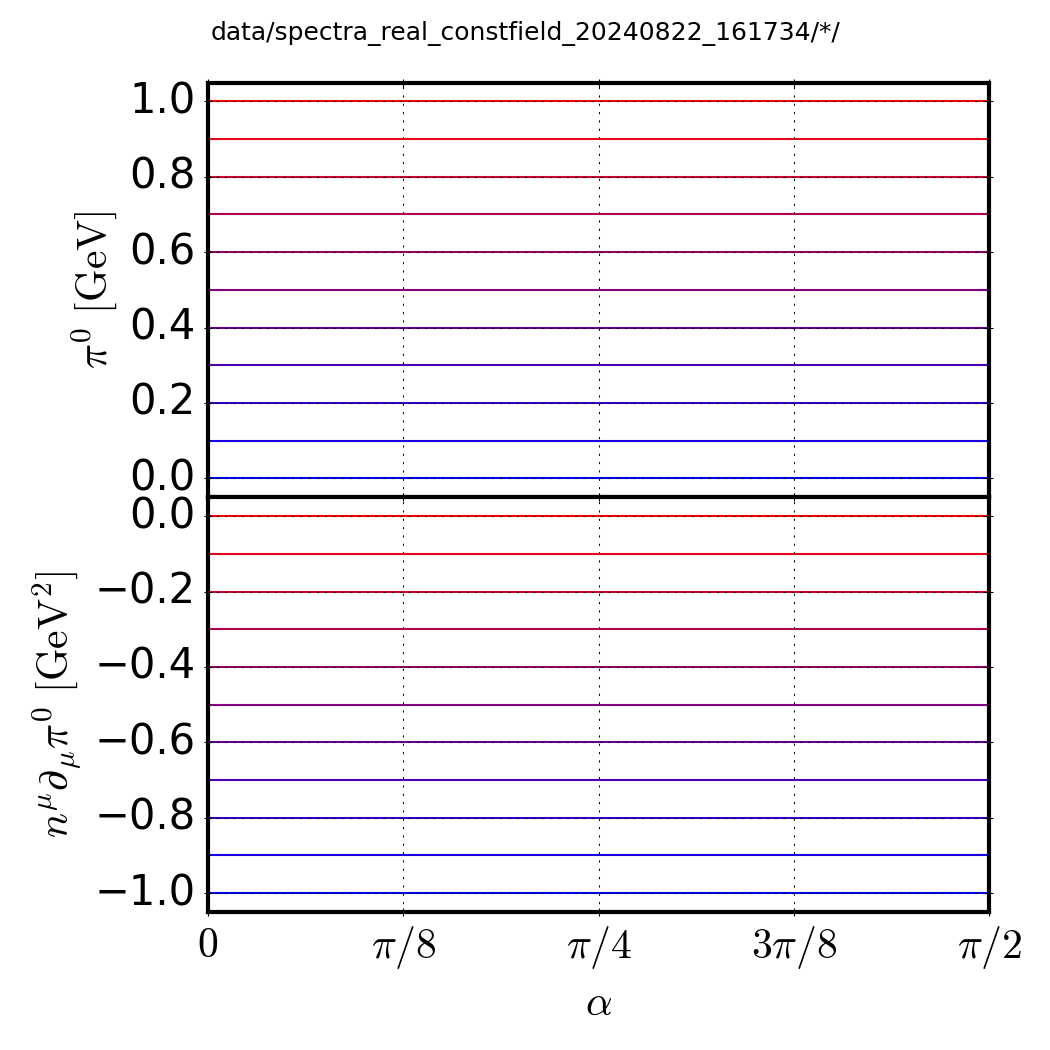
\includegraphics[width=\linewidth]{code/C++/DCCspec/data/images/spectra_real_constfield_20240822_161734_init.png}        
            \end{minipage}
        }
        \debugbox{
            \begin{minipage}{0.45\linewidth}
                \centering
                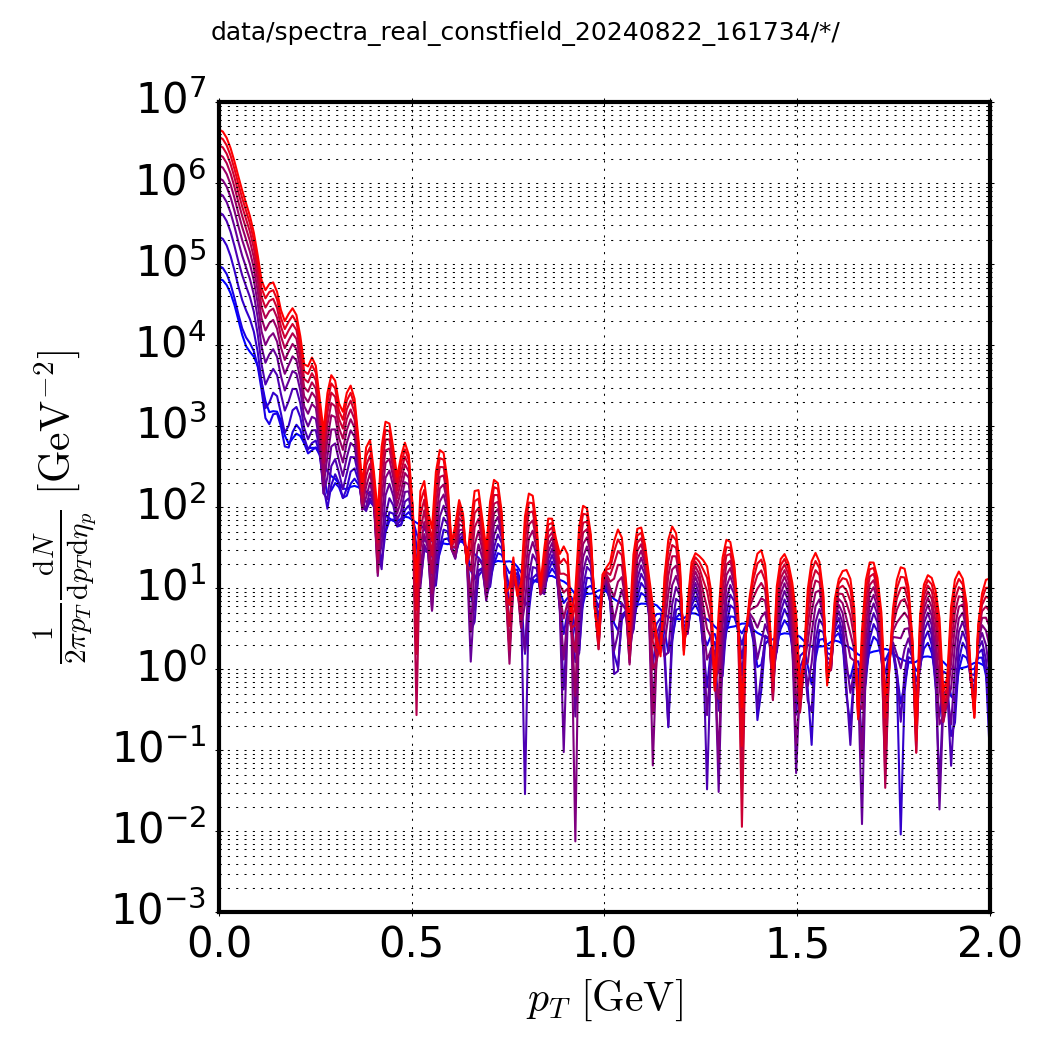
\includegraphics[width=\linewidth]{code/C++/DCCspec/data/images/spectra_real_constfield_20240822_161734_spec.png}        
            \end{minipage}
        }
    \end{minipage}
}
Spectra from field configurations of high ratio ${\Big\vert\frac{\text{amplitude}}{\text{derivative}}\Big\vert}$ tend to be more "bumpy"/oscillate quicker in momentum space.

These configurations are well suited to test separately the impact of the mass parameter in the spectrum computation, keeping the initial conditions fixed.\\
\debugbox{
    \begin{minipage}{\linewidth}
        \centering
        \debugbox{
            \begin{minipage}{0.45\linewidth}
                \centering
                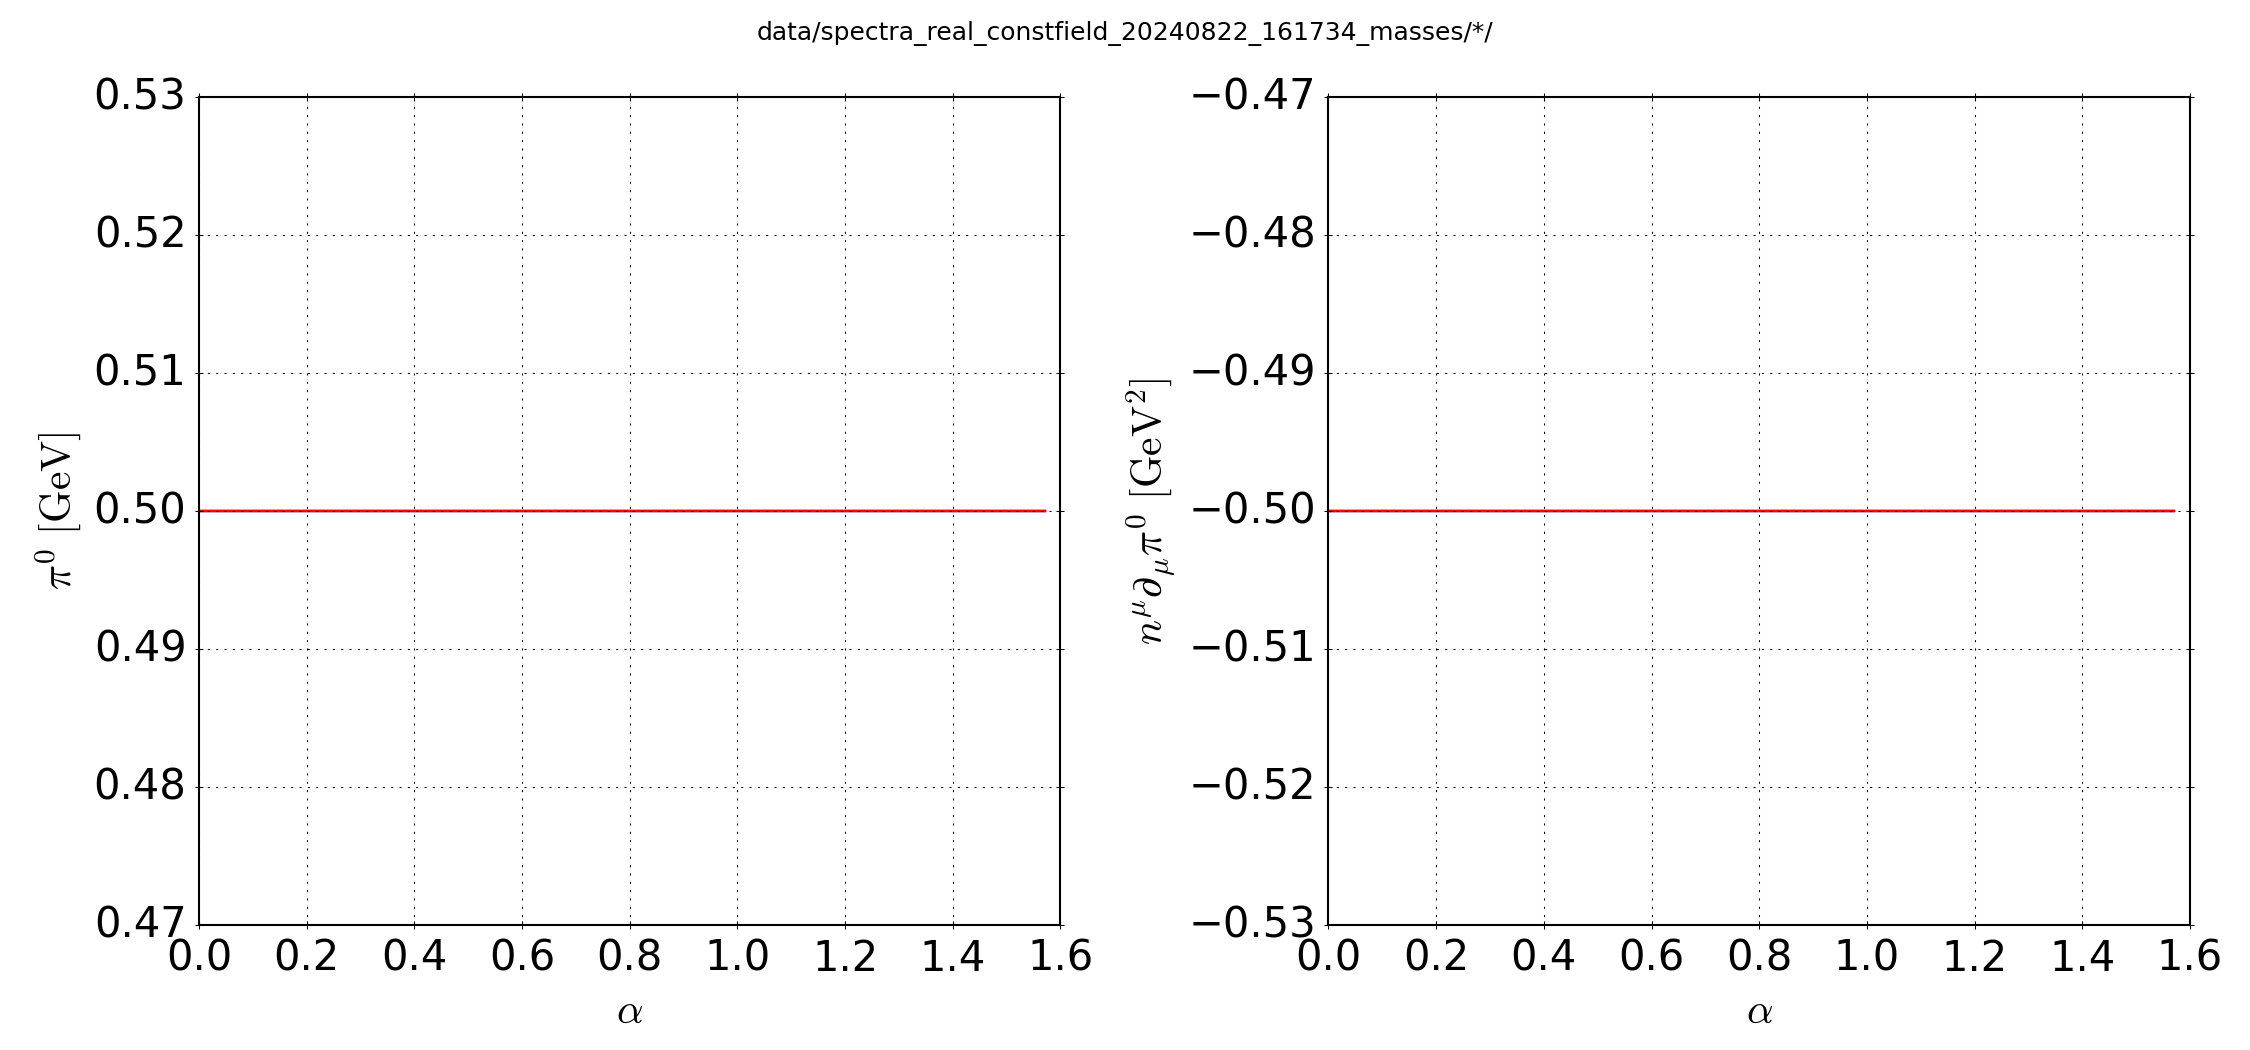
\includegraphics[width=\linewidth]{code/C++/DCCspec/data/images/spectra_real_constfield_20240822_161734_masses_init.png}        
            \end{minipage}
        }
        \debugbox{
            \begin{minipage}{0.45\linewidth}
                \centering
                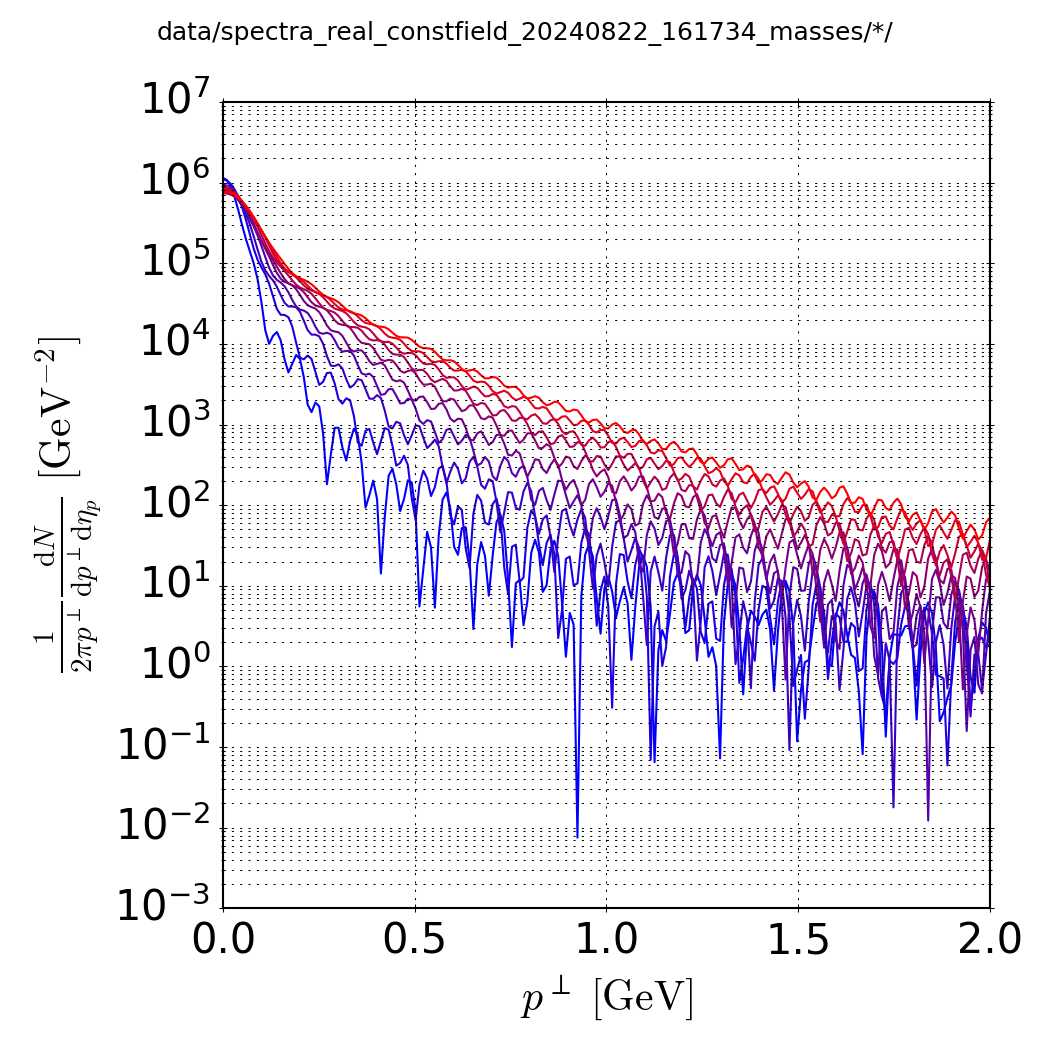
\includegraphics[width=\linewidth]{code/C++/DCCspec/data/images/spectra_real_constfield_20240822_161734_masses_spec.png}        
            \end{minipage}
        }
    \end{minipage}
}
The displayed graphs correspond to particle masses from 0.14 GeV (blue) to 0.8 GeV (red). Together with the scale on which the freezeout surface varies, the particle mass sets the main scale/width of the spectrum.


Next, test the $\epsilon=\const$ prescription of defining initial data, which yields a 1-parameter family of initial field configuration.\\
\debugbox{
    \begin{minipage}{\linewidth}
        \centering
        \debugbox{
            \begin{minipage}{0.45\linewidth}
                \centering
                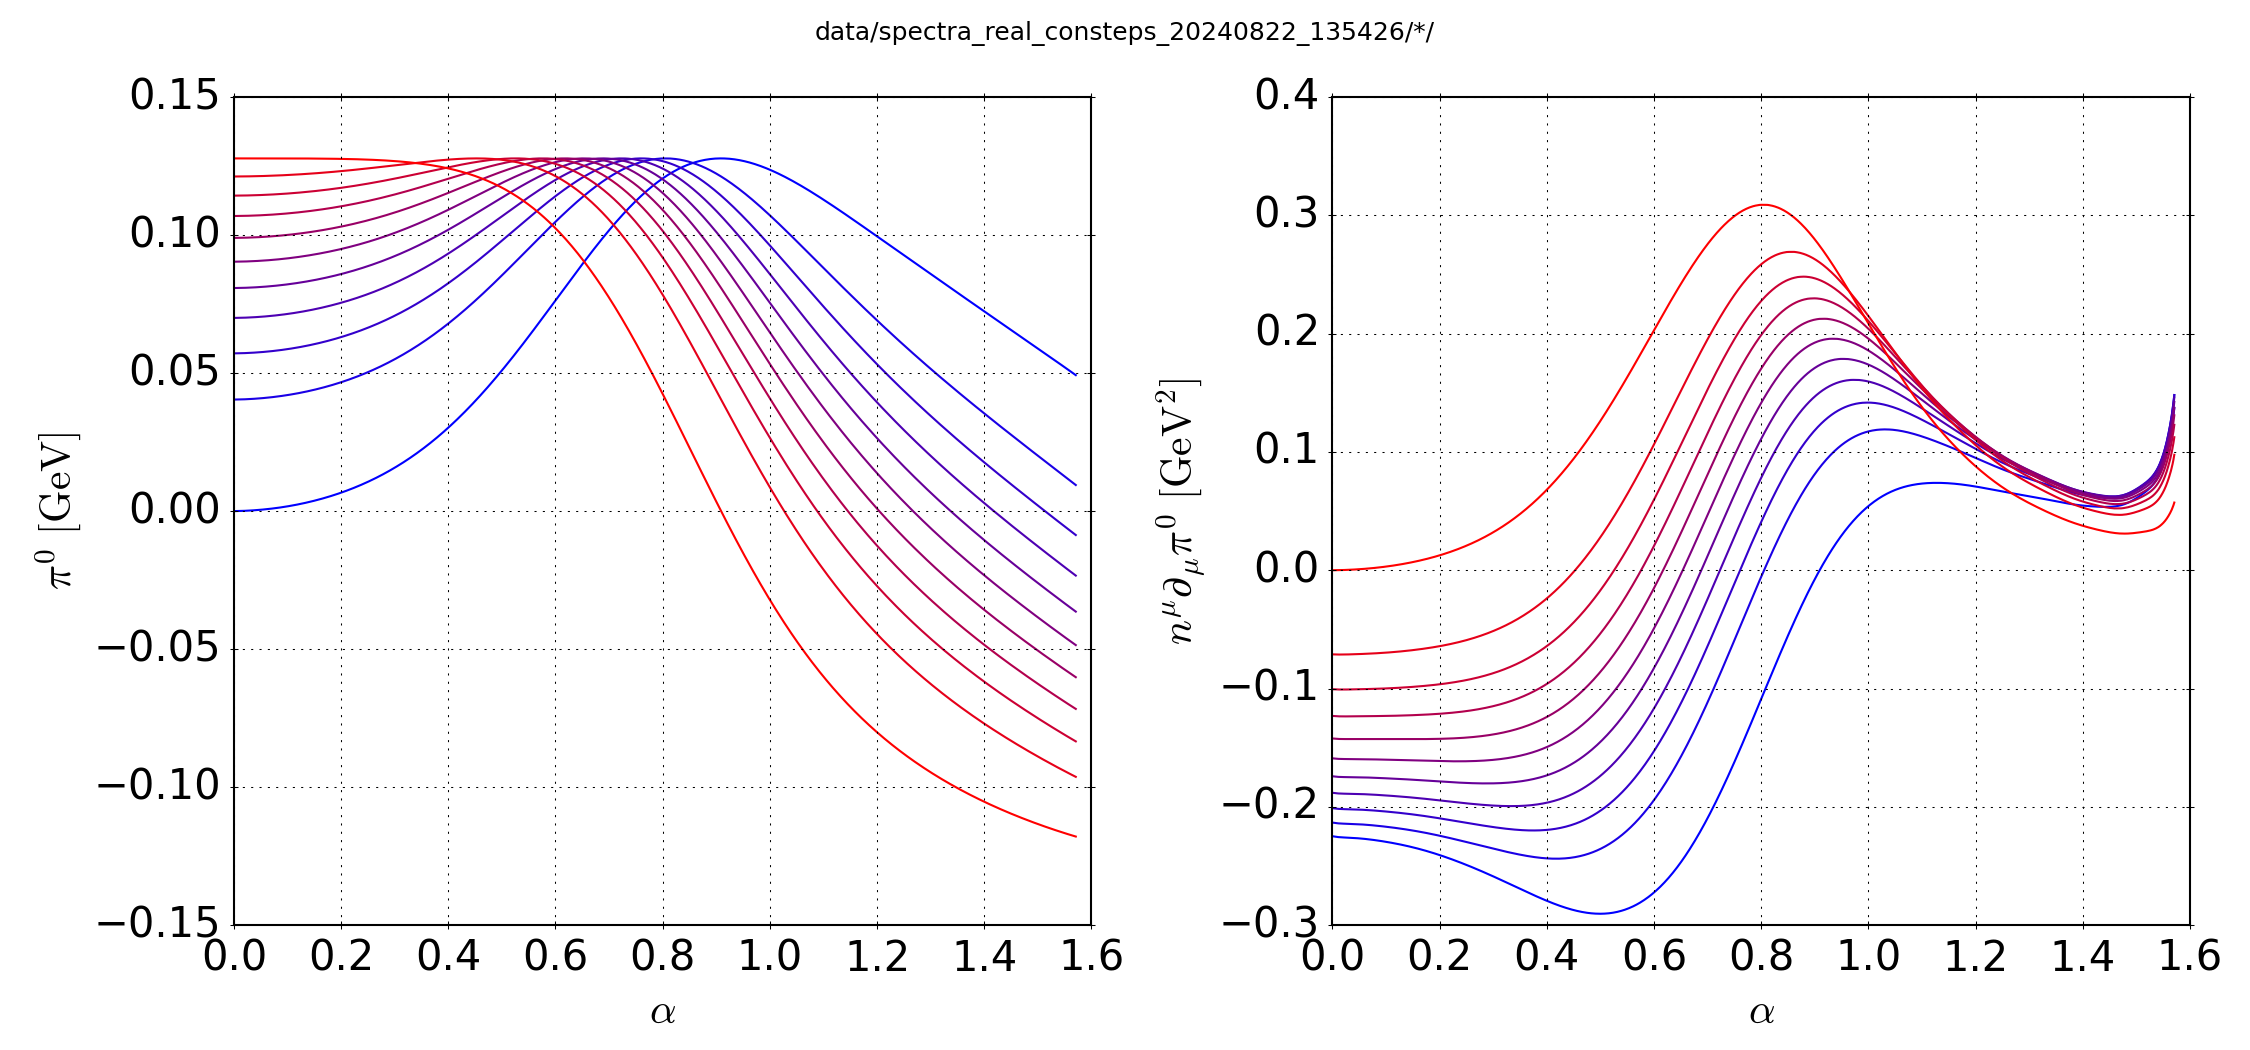
\includegraphics[width=\linewidth]{code/C++/DCCspec/data/images/spectra_real_consteps_20240822_135426_init.png}        
            \end{minipage}
        }
        \debugbox{
            \begin{minipage}{0.45\linewidth}
                \centering
                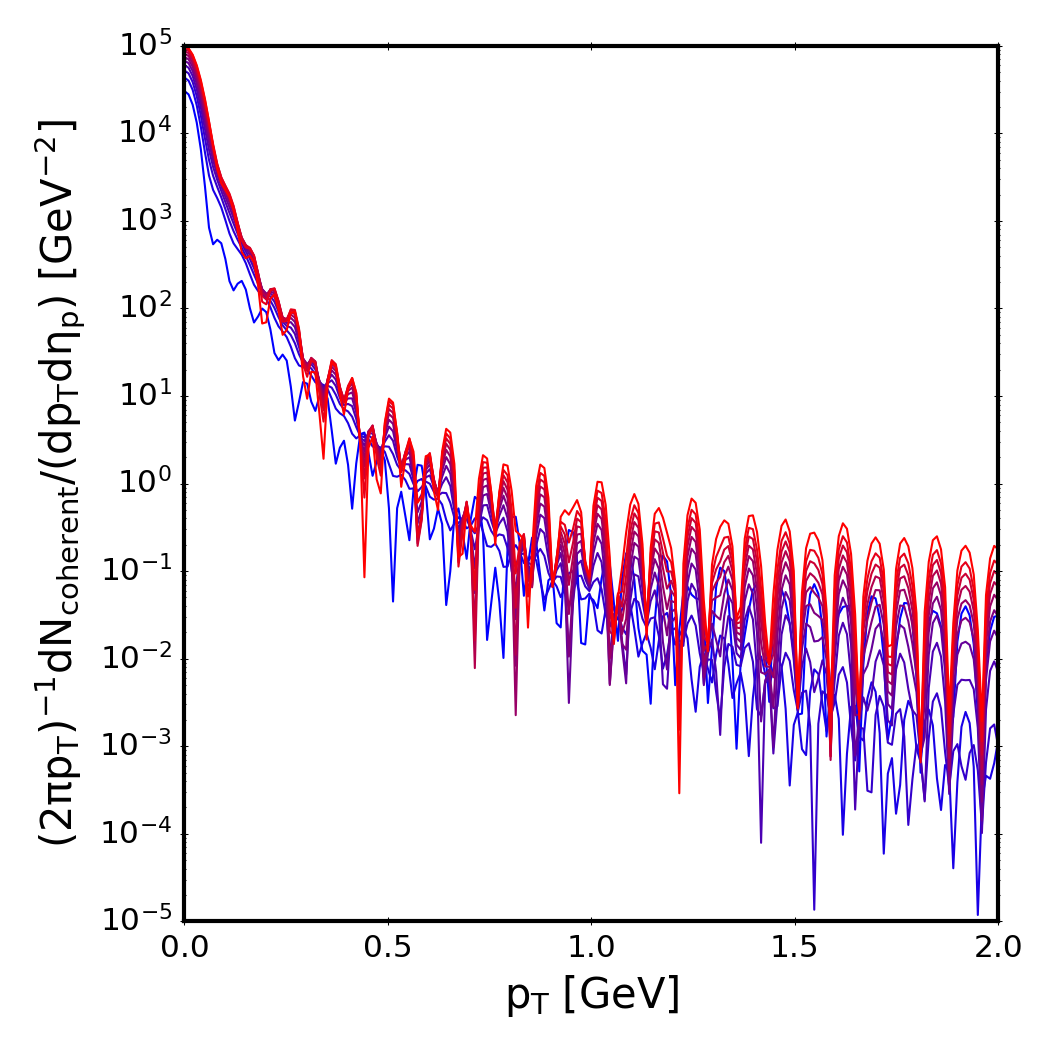
\includegraphics[width=\linewidth]{code/C++/DCCspec/data/images/spectra_real_consteps_20240822_135426_spec.png}        
            \end{minipage}
        }
    \end{minipage}
}
The red graphs represent field configurations that are approximately constant on the $\tau\approx\const$ section of the freezeout surface. They seem to generate a distinct "break" in the spectrum, where the average slope (in the log scale) changes abruptly.

Let us also change the mass in this scenario. Now, the mass also influences the initial conditions and lead to more oscillations along the freezeout surface. The following graphs range from 0.14 GeV to 1 GeV particle mass.\\
\debugbox{
    \begin{minipage}{\linewidth}
        \centering
        \debugbox{
            \begin{minipage}{0.45\linewidth}
                \centering
                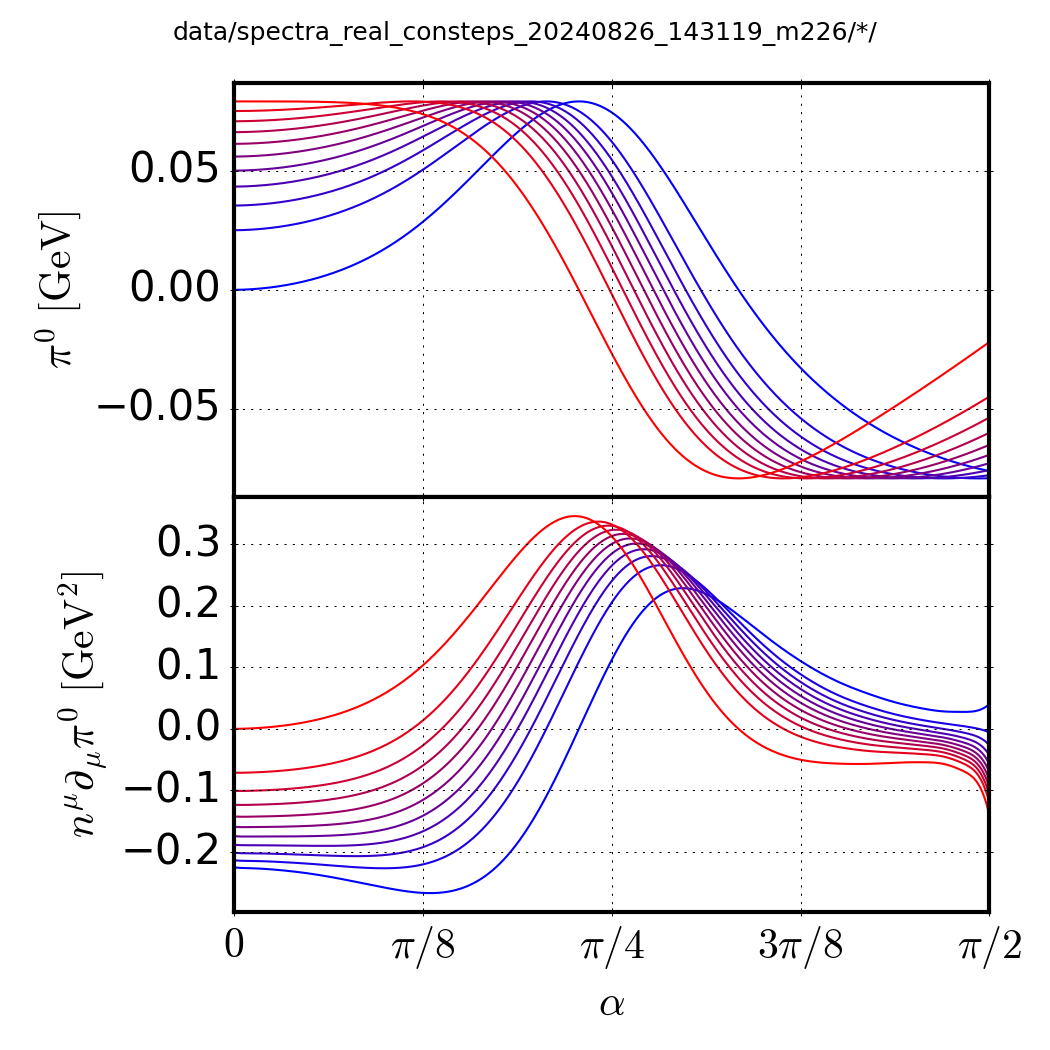
\includegraphics[width=\linewidth]{code/C++/DCCspec/data/images/spectra_real_consteps_20240826_143119_m226_init.png}        
            \end{minipage}
        }
        \debugbox{
            \begin{minipage}{0.45\linewidth}
                \centering
                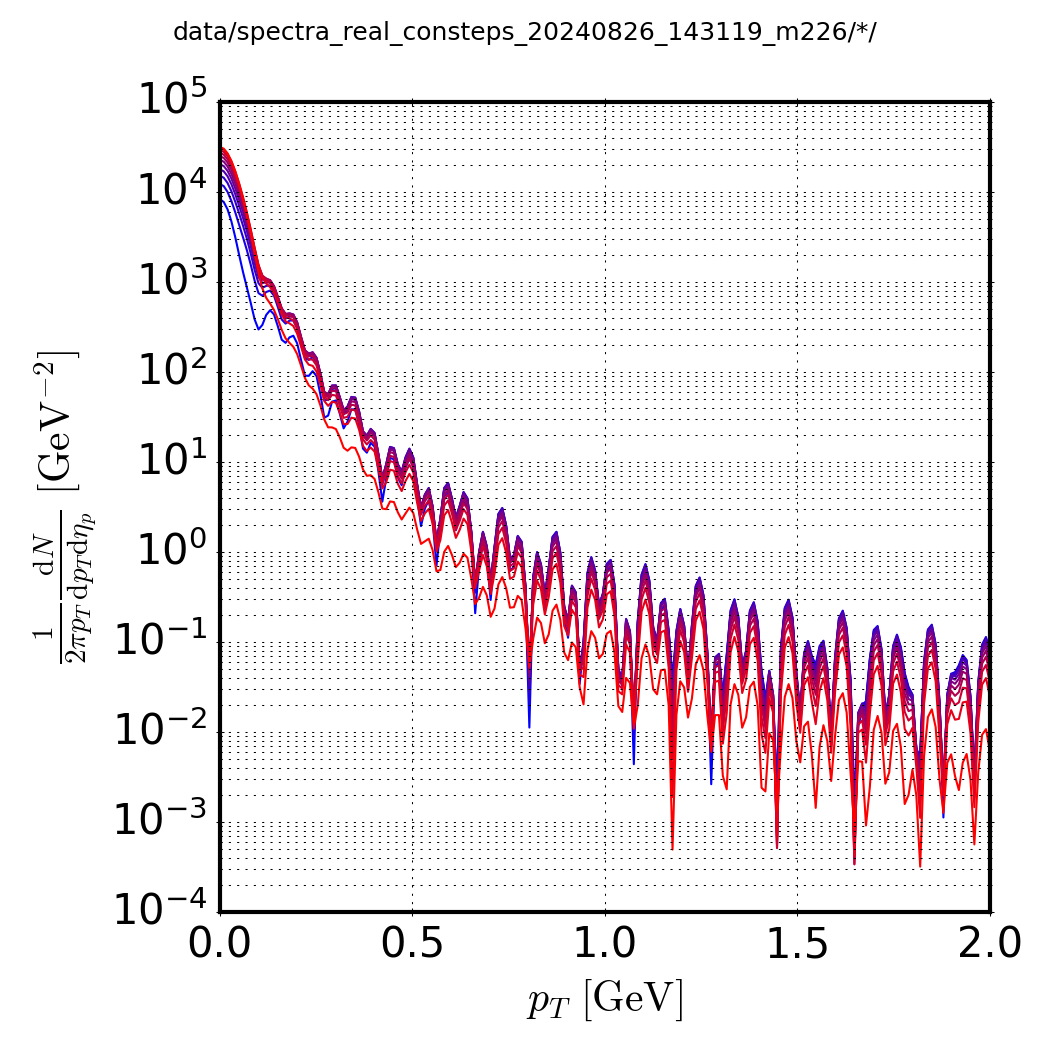
\includegraphics[width=\linewidth]{code/C++/DCCspec/data/images/spectra_real_consteps_20240826_143119_m226_spec.png}        
            \end{minipage}
        }
    \end{minipage}
}

\debugbox{
    \begin{minipage}{\linewidth}
        \centering
        \debugbox{
            \begin{minipage}{0.45\linewidth}
                \centering
                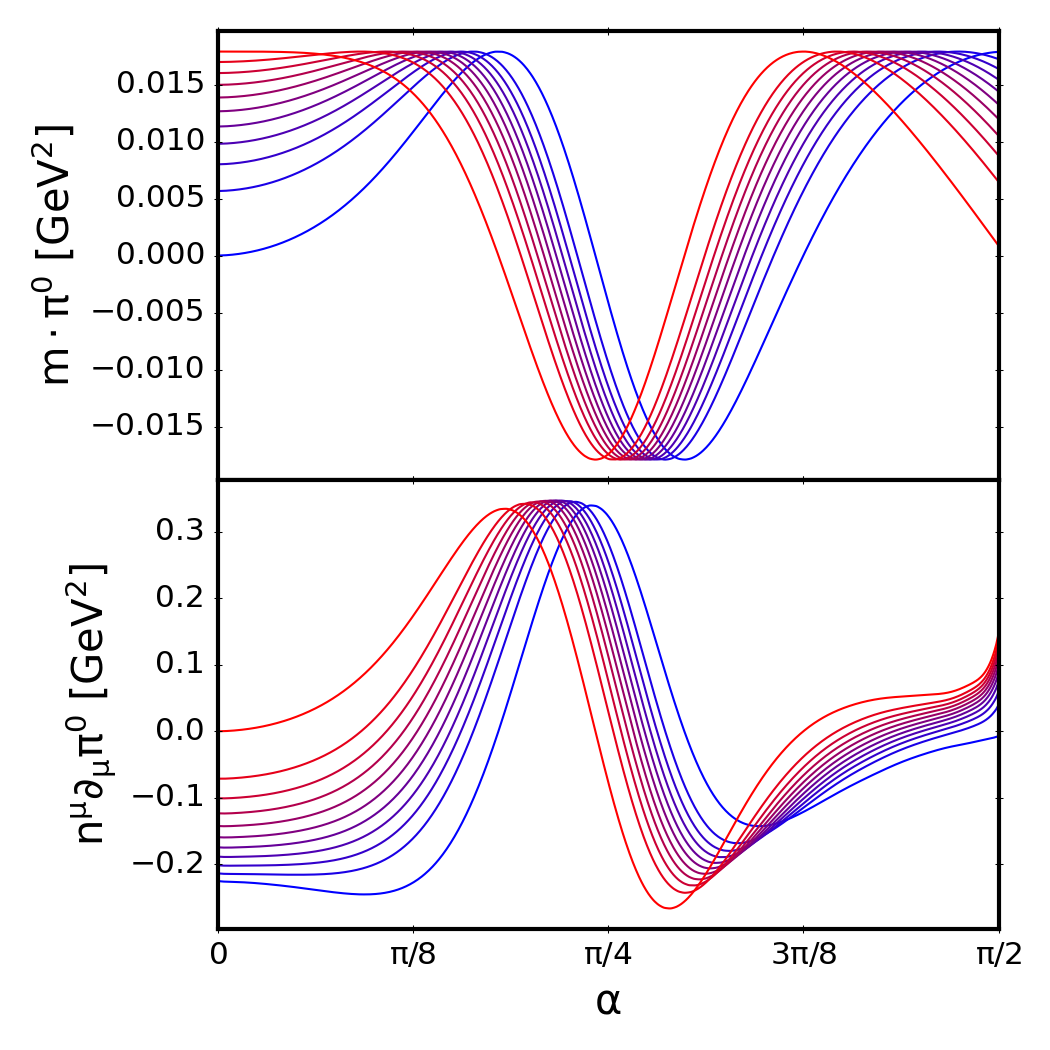
\includegraphics[width=\linewidth]{code/C++/DCCspec/data/images/spectra_real_consteps_20240826_143151_m398_init.png}        
            \end{minipage}
        }
        \debugbox{
            \begin{minipage}{0.45\linewidth}
                \centering
                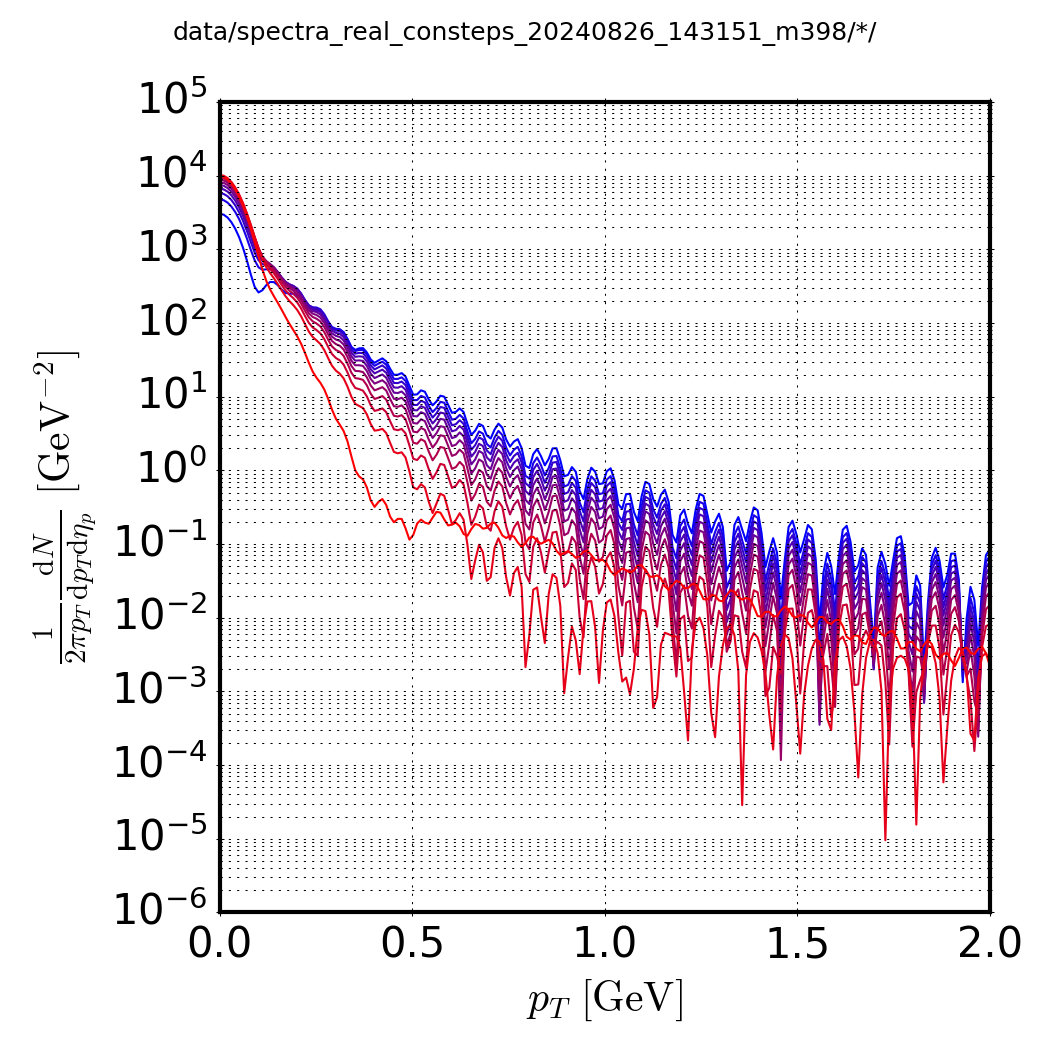
\includegraphics[width=\linewidth]{code/C++/DCCspec/data/images/spectra_real_consteps_20240826_143151_m398_spec.png}        
            \end{minipage}
        }
    \end{minipage}
}

\debugbox{
    \begin{minipage}{\linewidth}
        \centering
        \debugbox{
            \begin{minipage}{0.45\linewidth}
                \centering
                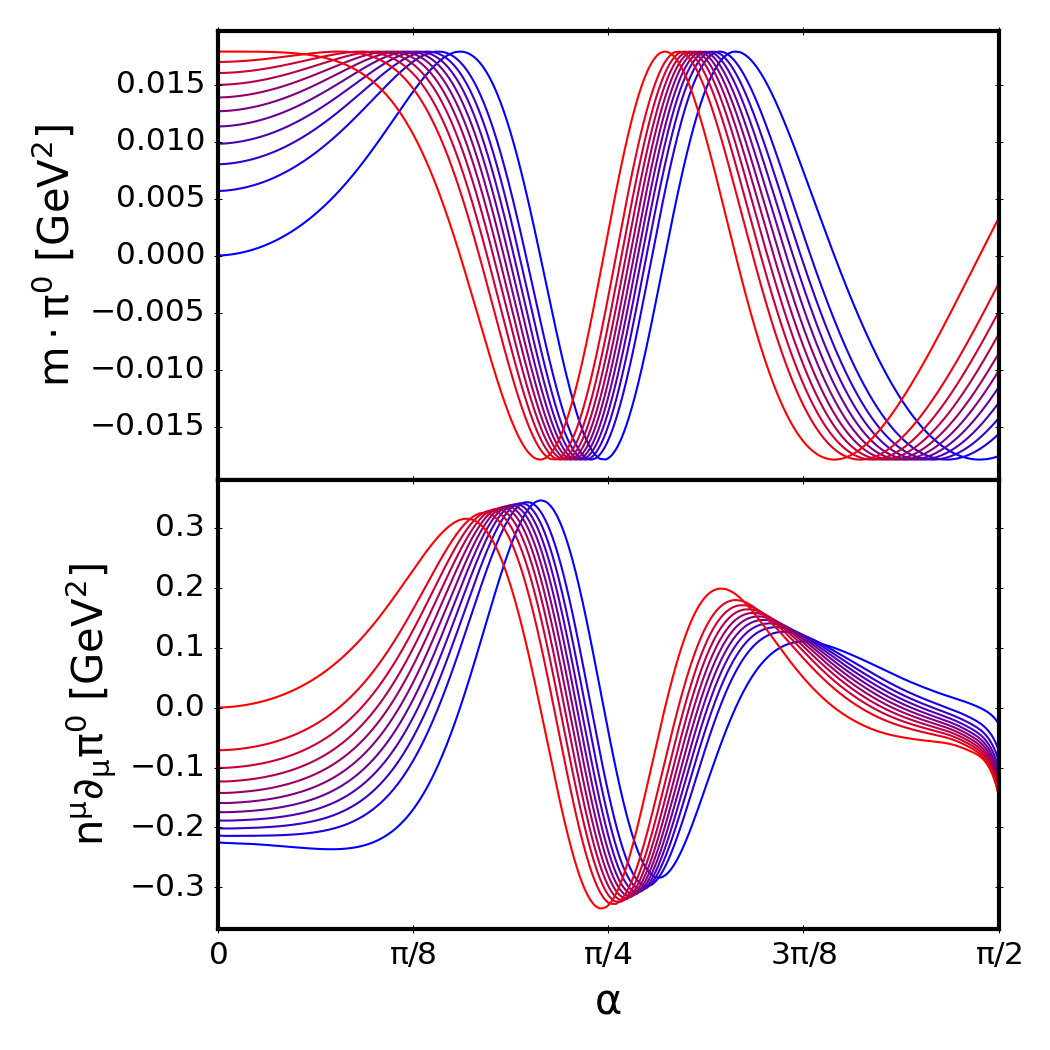
\includegraphics[width=\linewidth]{code/C++/DCCspec/data/images/spectra_real_consteps_20240826_143224_m570_init.png}        
            \end{minipage}
        }
        \debugbox{
            \begin{minipage}{0.45\linewidth}
                \centering
                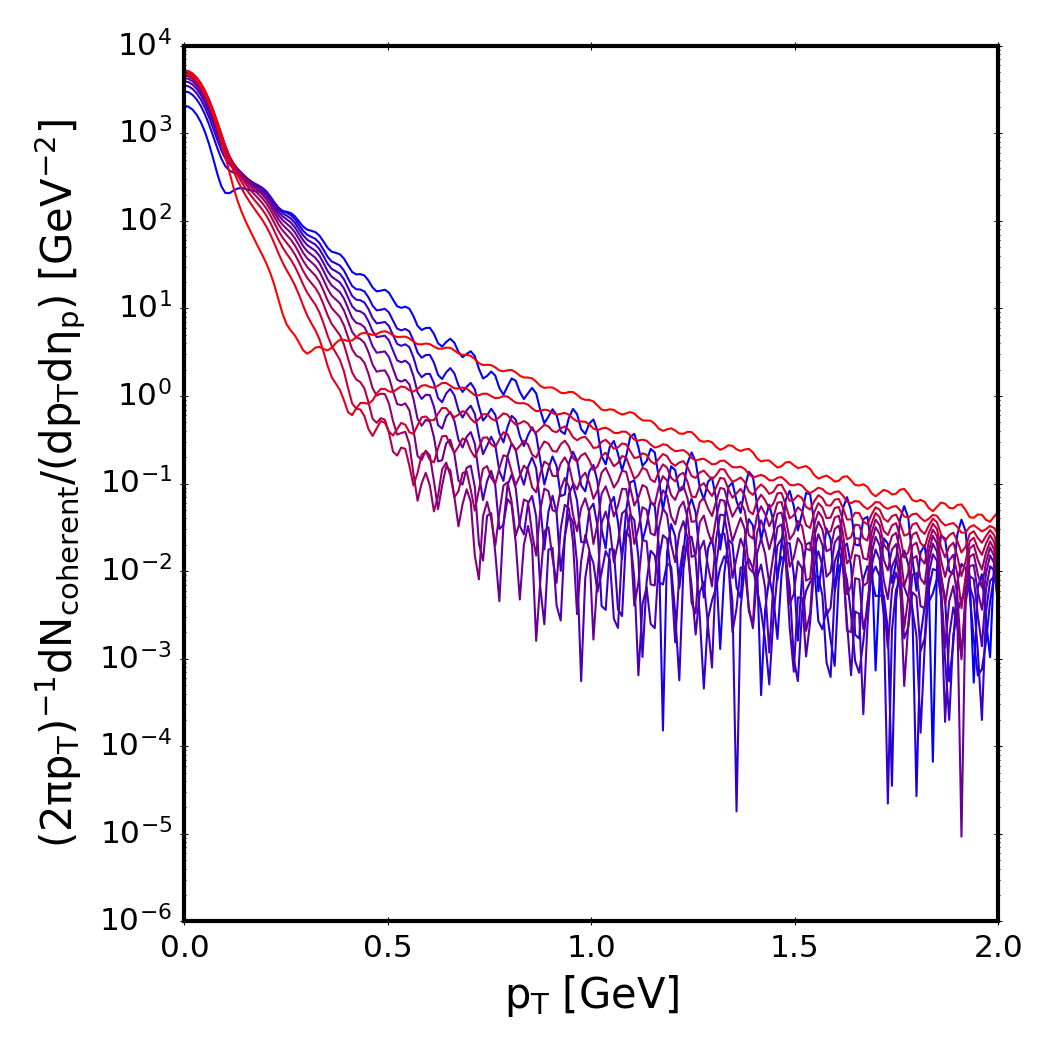
\includegraphics[width=\linewidth]{code/C++/DCCspec/data/images/spectra_real_consteps_20240826_143224_m570_spec.png}        
            \end{minipage}
        }
    \end{minipage}
}

\debugbox{
    \begin{minipage}{\linewidth}
        \centering
        \debugbox{
            \begin{minipage}{0.45\linewidth}
                \centering
                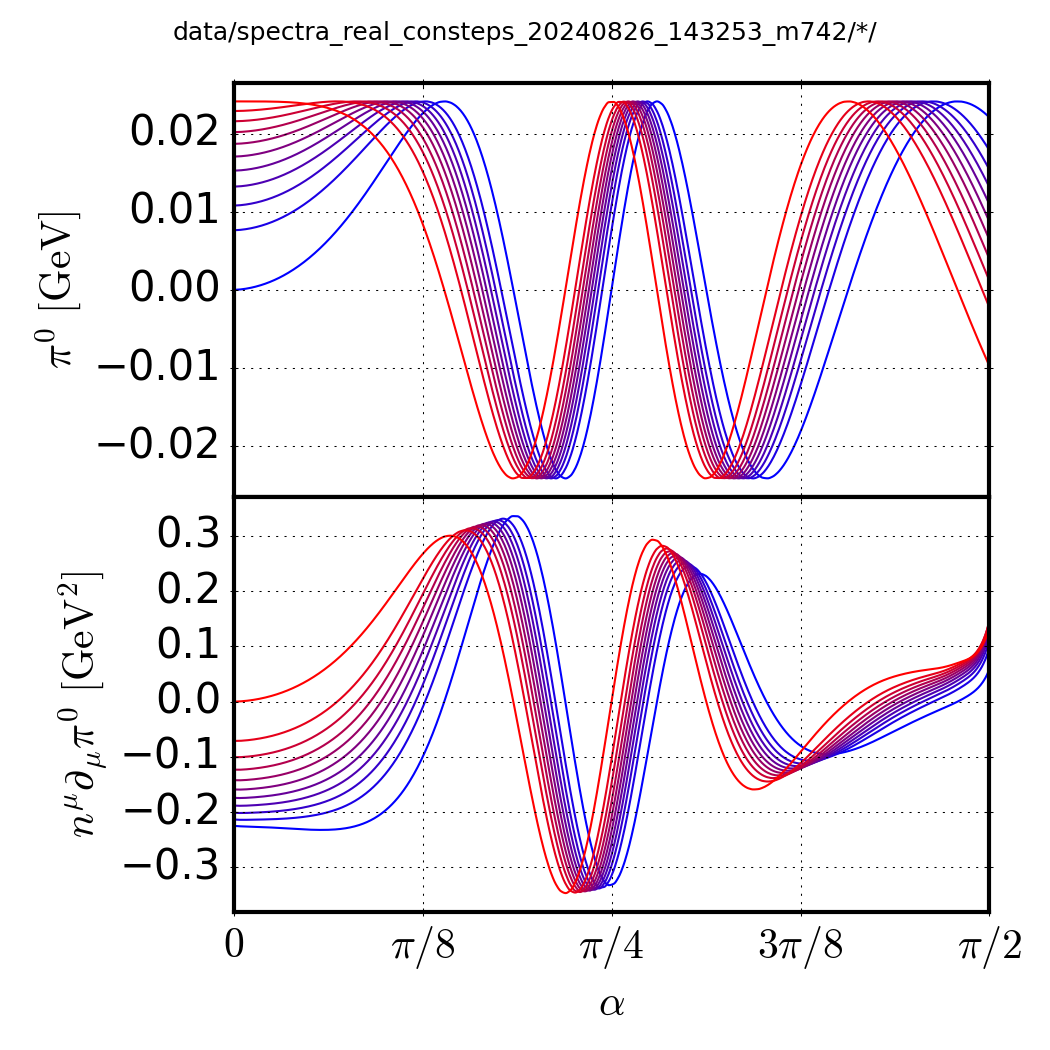
\includegraphics[width=\linewidth]{code/C++/DCCspec/data/images/spectra_real_consteps_20240826_143253_m742_init.png}        
            \end{minipage}
        }
        \debugbox{
            \begin{minipage}{0.45\linewidth}
                \centering
                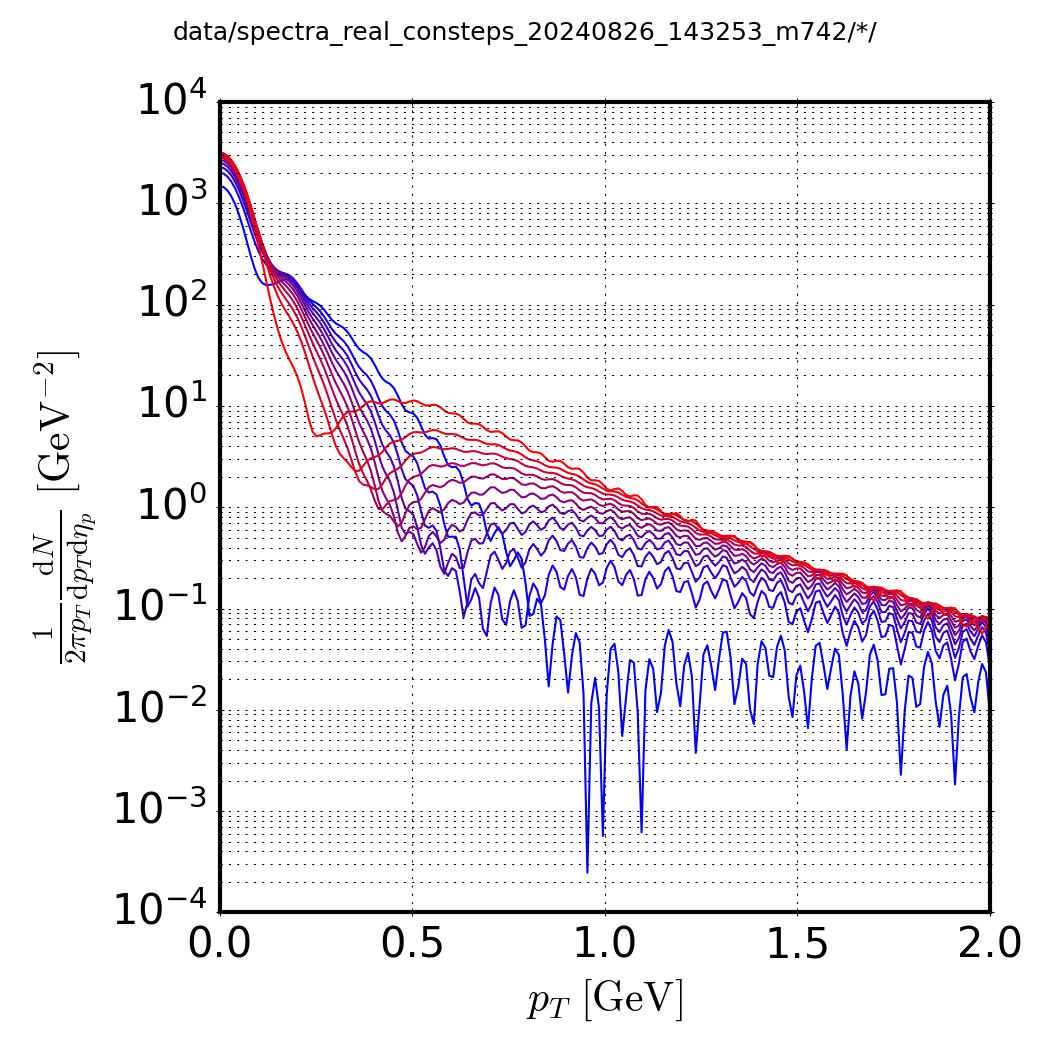
\includegraphics[width=\linewidth]{code/C++/DCCspec/data/images/spectra_real_consteps_20240826_143253_m742_spec.png}        
            \end{minipage}
        }
    \end{minipage}
}

\debugbox{
    \begin{minipage}{\linewidth}
        \centering
        \debugbox{
            \begin{minipage}{0.45\linewidth}
                \centering
                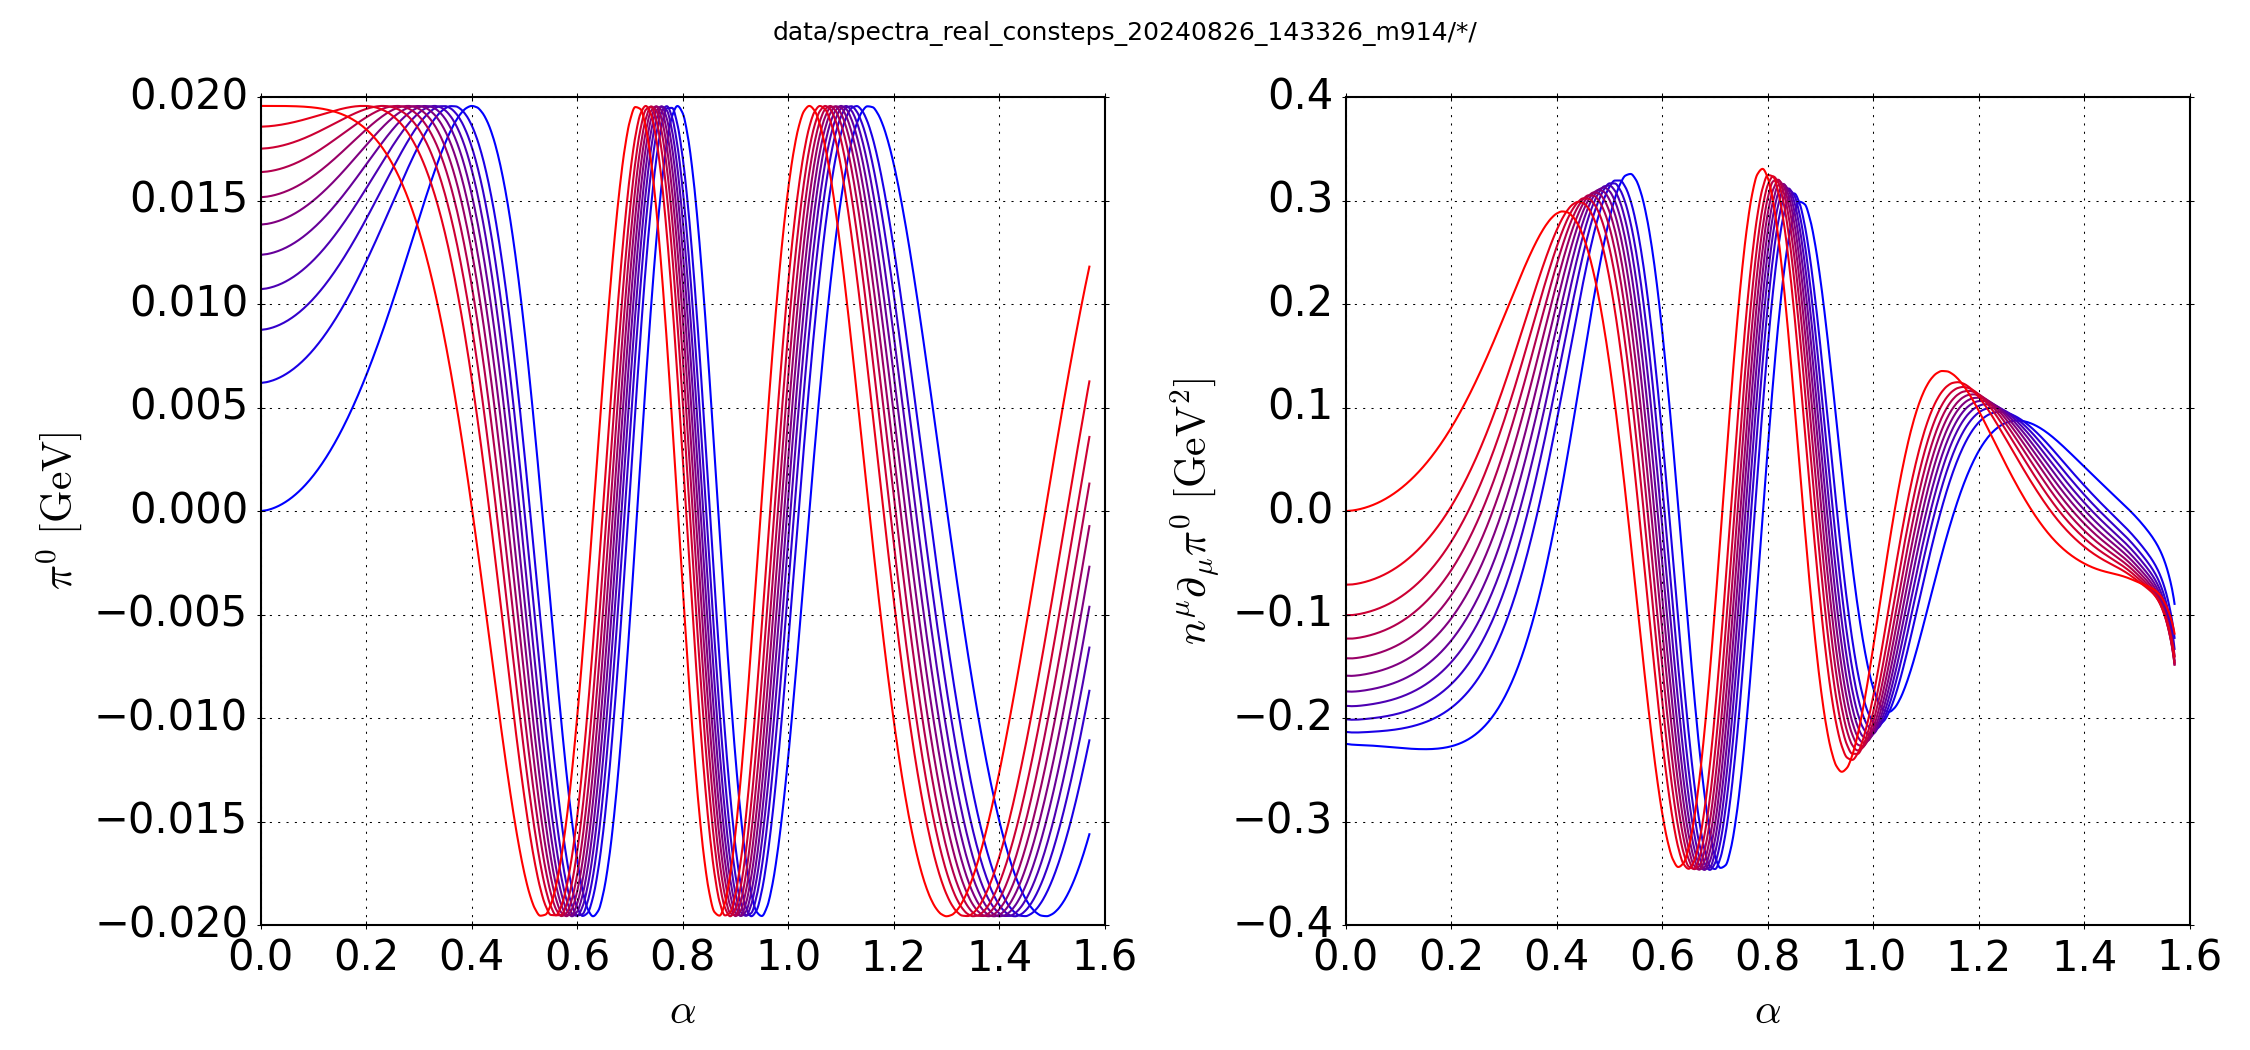
\includegraphics[width=\linewidth]{code/C++/DCCspec/data/images/spectra_real_consteps_20240826_143326_m914_init.png}        
            \end{minipage}
        }
        \debugbox{
            \begin{minipage}{0.45\linewidth}
                \centering
                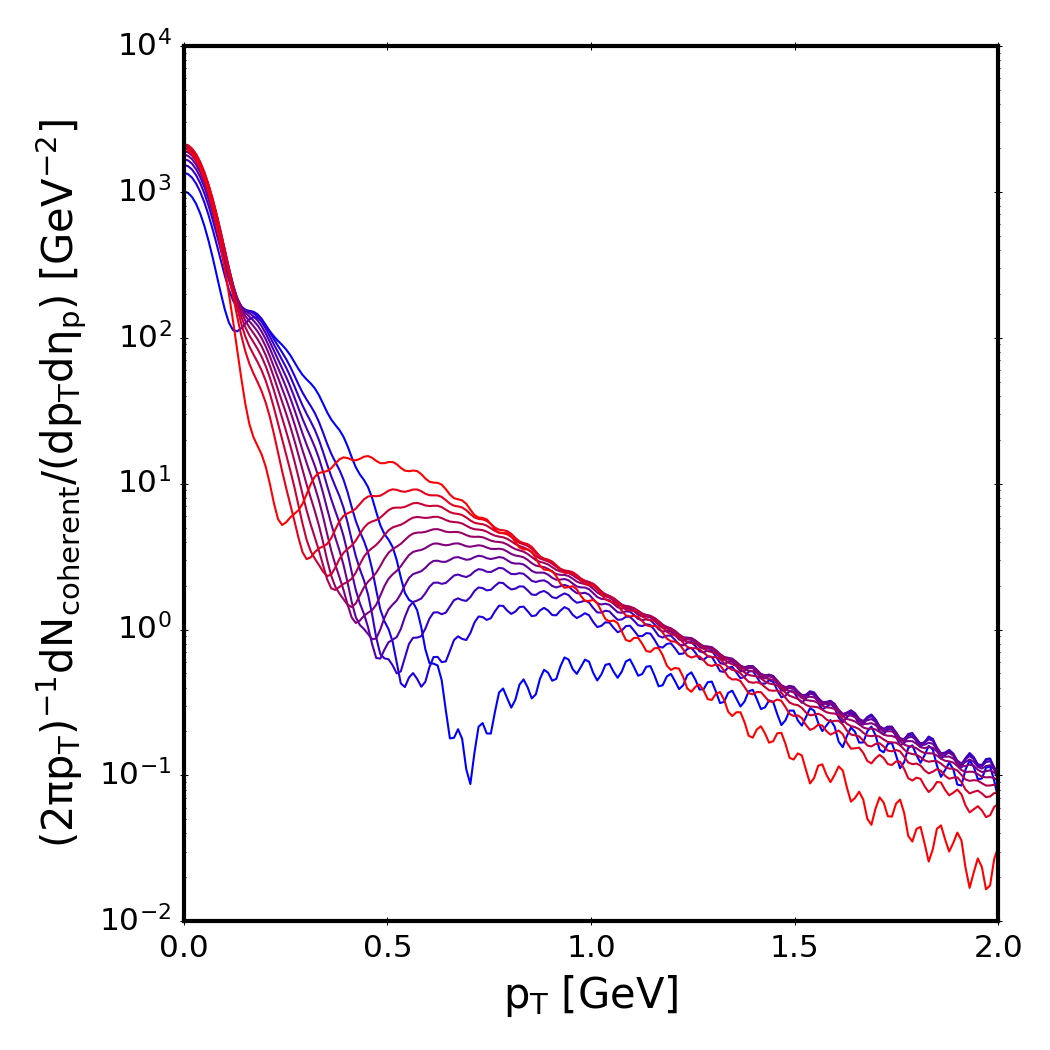
\includegraphics[width=\linewidth]{code/C++/DCCspec/data/images/spectra_real_consteps_20240826_143326_m914_spec.png}        
            \end{minipage}
        }
    \end{minipage}
}

\debugbox{
    \begin{minipage}{\linewidth}
        \centering
        \debugbox{
            \begin{minipage}{0.45\linewidth}
                \centering
                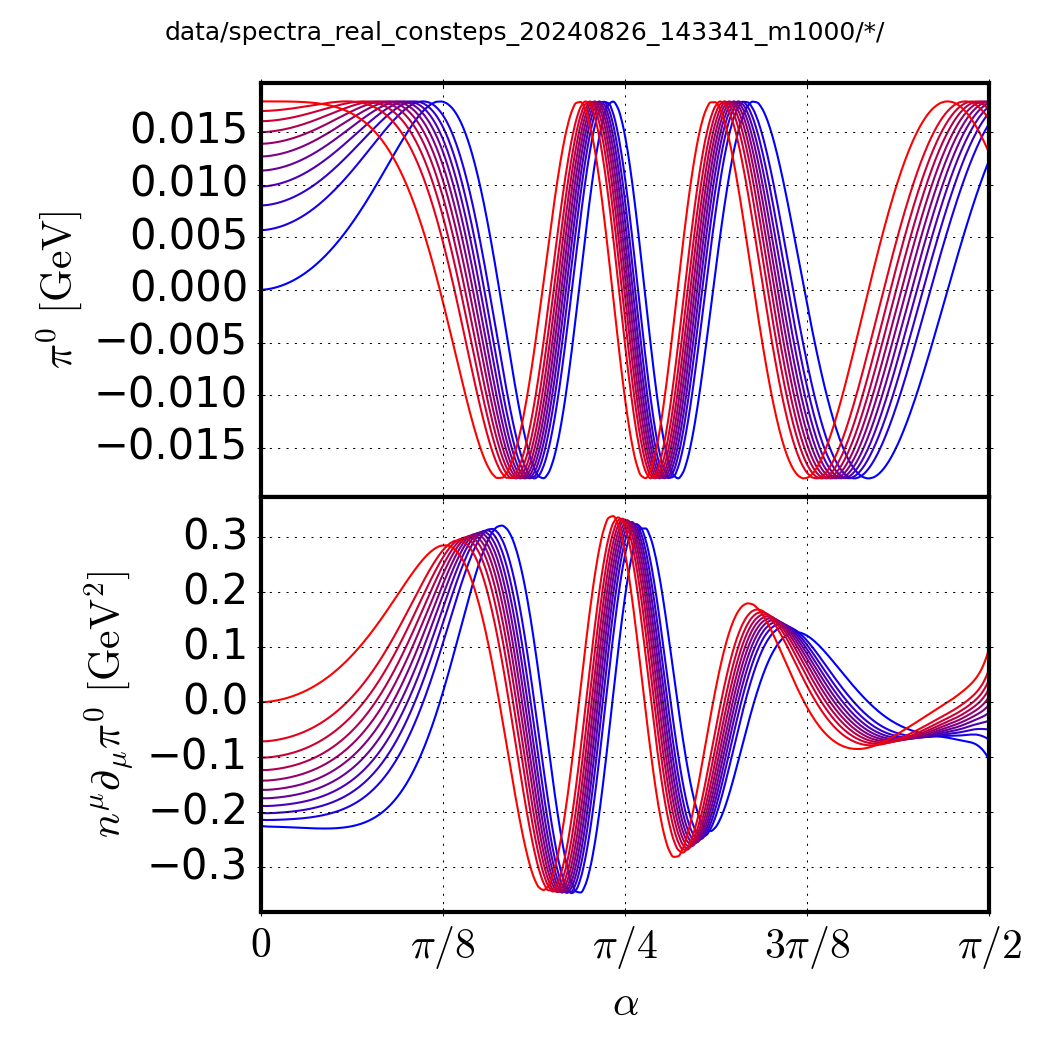
\includegraphics[width=\linewidth]{code/C++/DCCspec/data/images/spectra_real_consteps_20240826_143341_m1000_init.png}        
            \end{minipage}
        }
        \debugbox{
            \begin{minipage}{0.45\linewidth}
                \centering
                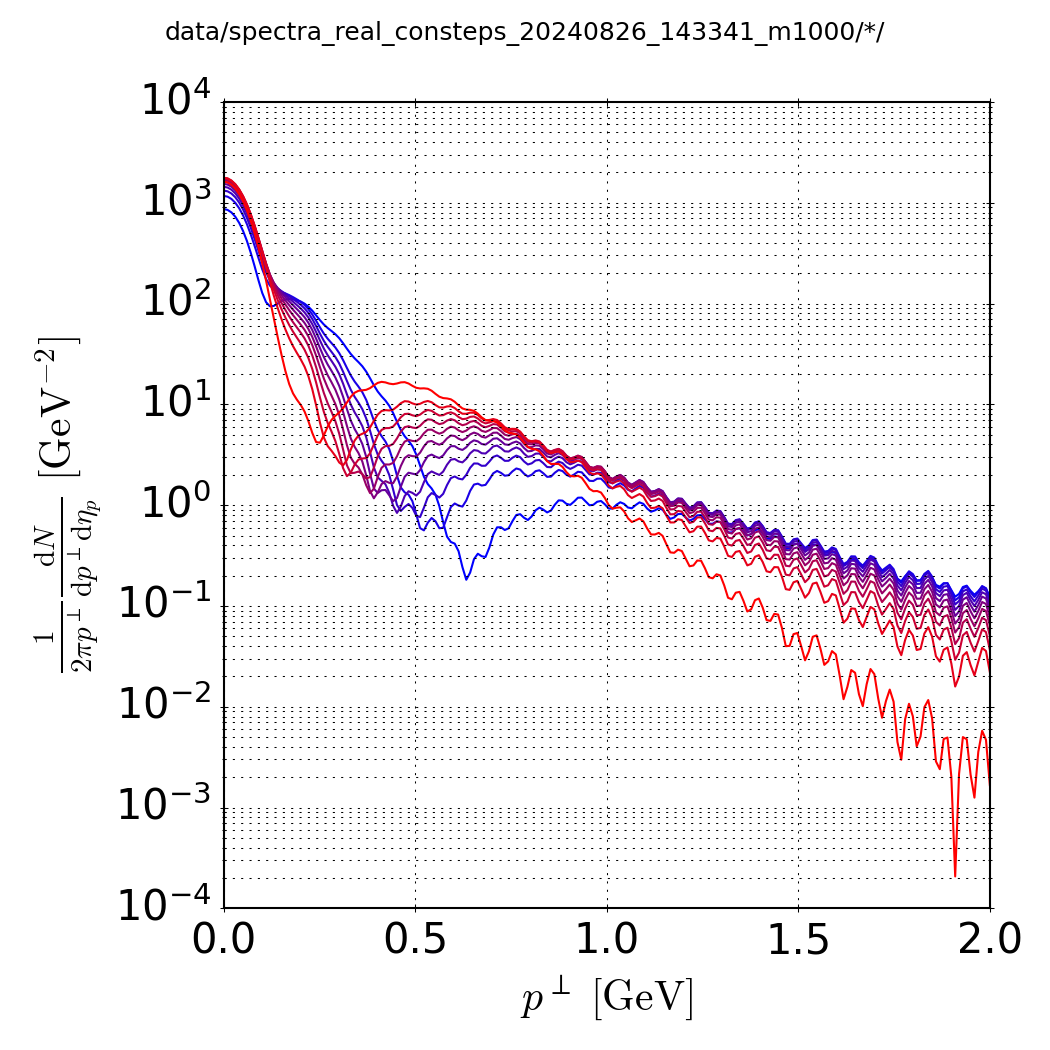
\includegraphics[width=\linewidth]{code/C++/DCCspec/data/images/spectra_real_consteps_20240826_143341_m1000_spec.png}        
            \end{minipage}
        }
    \end{minipage}
}
With increasing mass, one observers increasing width of the spectrum, as well as a second dominant bump away from $p=0\,\text{GeV}$, namely roughly at the particle mass.